\documentclass[12pt]{article} % Default font size is 12pt, it can be changed here

\usepackage{sectsty}
\usepackage{setspace}
\usepackage{titlesec}
\sectionfont{\fontsize{14}{15}\selectfont}
\subsectionfont{\fontsize{13}{15}\selectfont}
\titlespacing\section{0pt}{12pt plus 6pt minus 3pt}{6pt plus 4pt minus 2pt}
\titlespacing\subsection{0pt}{10pt plus 4pt minus 2pt}{6pt plus 2pt minus 2pt}
\titlespacing\subsubsection{0pt}{8pt plus 4pt minus 2pt}{2pt plus 2pt minus 2pt}

\usepackage{geometry} % Required to change the page size to A4
\geometry{a4paper} % Set the page size to be A4 as opposed to the default US Letter
\usepackage{graphicx} % Required for including pictures
\usepackage{float} % Allows putting an [H] in \begin{figure} to specify the exact location of the figure
\usepackage{wrapfig} % Allows in-line images such as the example fish picture
\usepackage{lipsum} % Used for inserting dummy 'Lorem ipsum' text into the template
\usepackage{listings}
\usepackage{color}
\usepackage{textcomp}
\usepackage{amsmath,amssymb,mathtools}
\usepackage{algorithm, algpseudocode}

\linespread{1.2} % Line spacing

%\setlength\parindent{0pt} % Uncomment to remove all indentation from paragraphs
\graphicspath{{Pictures/}} % Specifies the directory where pictures are stored
\usepackage{titlesec}

\setcounter{secnumdepth}{4}

\titleformat{\paragraph}
{\normalfont\normalsize\bfseries}{\theparagraph}{1em}{}
\titlespacing*{\paragraph}
{0pt}{8pt plus 3pt minus 2pt}{2pt plus 2pt minus 2pt}


\begin{document}

\definecolor{listinggray}{gray}{0.9}
\definecolor{lbcolor}{rgb}{0.9,0.9,0.9}

\lstset{backgroundcolor=\color{lbcolor},
	basicstyle=\ttfamily,
	tabsize = 4,
	columns=fixed,
	keywordstyle=\color[rgb]{0,0,1},
	showstringspaces = false,
	showspaces = false,
	commentstyle=\color[rgb]{0.133,0.545,0.133},
	%stringstyle=\color[rgb]{0.627,0.126,0.941}
}

\lstdefinestyle{appendix}
{backgroundcolor=\color{lbcolor},
	basicstyle=\tiny,
	tabsize = 4,
	columns=fixed,
	keywordstyle=\color[rgb]{0,0,1},
	numberstyle=\tiny\color{blue},
	numbers=left,
	showstringspaces = false,
	showspaces = false,
	commentstyle=\color[rgb]{0.133,0.545,0.133},
	%stringstyle=\color[rgb]{0.627,0.126,0.941}
}

%---------------
%	TITLE PAGE
%---------------
\begin{titlepage}

\newcommand{\HRule}{\rule{\linewidth}{0.5mm}} % Defines a new command for the horizontal lines, change thickness here

\center % Center everything on the page

\textsc{\LARGE Language for Linear Algebra}\\[1.0cm] % Name of your university/college


\begin{minipage}{0.4\textwidth}
\begin{flushleft} \large
\emph{Author:}\\
Chenzhe \textsc{Qian} \\
Guitian \textsc{Lan} \\
Jin \textsc{Liang} \\
Zhiyuan \textsc{Guo}
\end{flushleft}
\end{minipage}
~
\begin{minipage}{0.4\textwidth}
\begin{flushright} \large
\emph{UNI:} \\
cq2185 \\
gl2510 \\
jl4598 \\
zg2201
\end{flushright}
\end{minipage}\\[4cm]

{\large \today}\\[3cm] % Date, change the \today to a set date if you want to be precise

%\includegraphics{Logo}\\[1cm] % Include a department/university logo - this will require the graphicx package

\vfill % Fill the rest of the page with whitespace

\end{titlepage}


\tableofcontents
\newpage

\section{Introduction}
\noindent The Language for Linear Algebra (LFLA) is a multi-paradigm and domain-specific programming language. It is focused on linear algebra programming and mainly designed for educational purpose. This language will help linear algebra learner to have a clear understanding of linear algebra concepts and terminologies, and use the language for computation. The input language of LFLA syntactically resembles the Matlab programming language. The output of the translator is Python code with a built-in library, compiles to an executable python script. LFLA inherits the benefits of functional programming language and powered by object-like primitive types (see Features). LFLA makes linear algebra calculation easy to code, read and understand. Besides, LFLA's syntax resembles common imperative languages so that makes programmers be comfortable to build complex programs.


\subsection{Background}
\noindent Linear algebra programming, though can be done by many existed languages such Matlab, R, Maple and etc, is still confusing on the concept-level. For example, none of the modern suitable languages clearly separates the concept of vector and matrix. Learners, even experienced programmers, may consider a matrix consists of vector(s). Such misunderstanding may not affect too much on industrial-orientated environment but will significantly mislead students to catch its essence. \\

\noindent We believe that computer science should play a crucial role in math education especially helping students to learn tough subjects like linear algebra. A good linear algebra programming language should not only do computing, but also help the students comprehend the fundamentals and the beauty of the linear algebra. Given this situation, we would like to create a domain language to help students and teachers in learning and teaching linear algebra. The Language for Linear Algebra(LFLA) is mainly designed for educational purpose.

\subsection{Features} 
\noindent LFLA introduces several primitive types direct corresponding to the concepts in linear algebra. Except as the matrix, it has vector, vector space, affine spaces and inner product space as primitive types. Besides the basic matrix calculation, LFLA emphasizes the relation between vector space, vectors and matrix (considered as a map). LFLA also incorporates the formal math notations into its language syntax to be consistent with math language.

\subsection{Related Work}
\noindent As mentioned in above, many modern programming languages support linear algebra programming. Matlab is known for its easiness to represent matrix and python is good for logical design and function building. LFLA mixes the syntax of Matlab and Python and is uniquely designed on the concepts of linear algebra. The built-in library that performs complicated calculations is implement in Python.






%-------------------
\section{Tutorial}
\subsection{Compile the program}
\noindent Our compiler is named LFLA, which stands for language for linear algebra. So for the program file name, it should have postfix .la, as a indication of LFLA language. Here is a sample program.
 \begin{lstlisting} 
#filename: sample.la
function main()
{
	print(1);
}
 \end{lstlisting}
In sample.la, we only have one main function, which is the execution start of the program. In main function, it calls a builtin function print.\\
To compile sample.la file, specify the input file and output file to the compiler:
\begin{lstlisting} 
> ./LFLA sample.la -o sample
\end{lstlisting}
If you don't specify output file name, compiler will generate an a.out file:
\begin{lstlisting} 
> ./LFLA sample.la 
\end{lstlisting}
Then execute the output file and get the results:
\begin{lstlisting} 
> ./sample
1
\end{lstlisting}
\subsection{Write the program}

\subsubsection{Date types}
\noindent LFLA has 6 primitive data types, which are:\\
\textbf{var}  \quad  \textbf{vector} \quad \textbf{matrix}  \quad\textbf{vecspace} \quad\textbf{ inspace} \quad \textbf{affspace} \\
It also supports the array data structures for each type. For array declaration, it should specify the length of array explicitly. 
\begin{lstlisting}
# types.la
function main()
{
	var a = 1;
	vector 	 b = [1,2,3];
	vector 	 c[2] = {[1,0], [0,1]};
	matrix 	 d = [1,2;3,4;];
	vecspace e = L([1,2], [4,5]);
	inspace  f = inspace({[1,0],[0,1]}, c);
	affspace g = affspace(b,d);
	print(a);
	print(b);
	print(c);
	print(d);
}
\end{lstlisting}
Compile the program and execute:
\begin{lstlisting} 
> ./LFLA types.la
> ./a.out
1
[1 2 3]
[array([1, 2]), array([3, 4])]
[[1 2]
[3 4]]
\end{lstlisting}	
\subsubsection{Control flows} 
\noindent LFLA supports 3 common control flows, which are if, while and for.The syntax for each one is as follows:
\begin{lstlisting} 
#if statements
if expression { }
# while statements
while expression { }
# for loop
var a;
for a = n1:n2 { }
\end{lstlisting}
\subsubsection{Define functions}
\noindent To define a function in LFLA, it should start with a reserved word function, then follows the name of function. And every program should have a main function, which is the execute start of the program.
\begin{lstlisting} 
# function.la
function foo(var a) {	
	print(a);	
}

function main() {
	foo(10);
}
\end{lstlisting}
Compile and execute:
\begin{lstlisting} 
> ./LFLA function.la
> ./a.out
10
\end{lstlisting}
\subsubsection{Built-in functions} 
\noindent To help programmar better use this language, LFLA provide several built-in functions. Here is a list of built-in functions:\\
\textbf{ceil}  \quad  \textbf{floor} \quad \textbf{sqrt}  \quad\textbf{dim} \quad\textbf{size}\quad\textbf{basis} \quad \textbf{rank} 
\quad \textbf{trace} \quad \textbf{eigenValue}\\
\subsubsection{Combine together} 
\noindent Combine all these together, we can acheive some wonderful work using LFLA. Here is a sample code checking the linear independence of an array of vectors.
\begin{lstlisting} 
# sample1.la
function linearIndep(vector[] vectors, var n)
{
	if n==1 { return 1; }
	if n > dim(vectors[0])
		{ return 0; }

	vecspace vs;
	var i;
	for i = 0:n
	{
		if vectors[i]@vs
			{return 0;}
	vs = vs + L(vectors[i]);
	}

	return 1;
}
function main()
{
	vector v = [1,2,3];
	vector u = [2,22,3];
	vector w = v + u;
	vector x[2] = { v, u};
	vector y[3] = {v, u, w};

	print(linearIndep(x, 2));

	print(linearIndep(y, 3));
}
\end{lstlisting}
Compile and execute:
\begin{lstlisting} 
> ./LFLA sample1.la
> ./a.out
1
0
\end{lstlisting}
\section{Language Reference Manual}
\subsection{Introduction}
This manual describes LFLA, a imperative programming language.  LFLA is
designed to  simulate the theory. Features defining the language
include  various primitive types and operations  corresponding to important concepts and theory  of  linear algebra. This manual
describes in detail the lexical conventions, types,  operations , built-in functions, and grammar of the LFLA
language.


\subsection{Lexical conventions}

\subsubsection{Identifiers}
An identifier in LFLA represents a name for functions or variables. The identifier starts with a letter, and is optionally followed by letters, digits or underscores. An identifier name is thus defined
by the following regular expression:  
  \newline
['a' - 'z' 'A' -'Z' ] ['a' - 'z' 'A' - 'Z' '0' - '9' '\_']*

\subsubsection{Keywords}
LFLA has a set of reserved keywords that can not be used as identifiers.
\paragraph{Types} Each primitive type, var, vector, vecspace, inspace,affspace and matrix, has a name that the program
uses for declarations:\\
 \textbf{var}  \quad  \textbf{vector}  \quad\textbf{vecspace} \quad\textbf{ inspace} \quad \textbf{affspace} \quad \textbf{matrix}
 \paragraph{Function}The keyword for declaration of  function:\\
\textbf{function}
\paragraph{Entry point of the program}  The keyword  for indication of  entry function :\\ 
\textbf{main}
\paragraph{Control flow}The following keywords are used for control flow:\\
 \textbf{if}\quad \textbf{else} \quad\textbf{for}\quad\textbf{while}\quad\textbf{break}\quad\textbf{continue}\quad\textbf{return}

\paragraph{Built-in functions} The following keywords are reserved for built in functions:\\
\textbf{print}\quad \textbf{dim} \quad \textbf{basis}\quad \textbf{sqrt} \quad \textbf{ceil} \quad \textbf{floor}\quad \textbf{size}\quad \textbf{rank}\quad \textbf{trace}
\quad\textbf{eigenValue}\quad\textbf{solve}\quad \textbf{image} \quad\textbf{L} 

\subsubsection{Constants}
LFLA supports integer, double as well as vector, matrix constants.   
\paragraph{Integer}  In LFLA an integer  is a signed 31-bit  integer without decimal point or exponent. It is given by  the following regular expression:
\newline
 [+ - ][ '0' -  '9 ']+
\paragraph{Double} In LFLA a double is a64-bit floating point number. More precisely it has an integral part, a fraction part and an exponent part. The integral part can begin with an optional '+' or '-', then follows by digits. And if it is not zero, the first digit should not be '0'. The fraction part is just a decimal followed by a finite sequence of digits . The exponent part begins with 'e' or 'E', then followed by an optional '+' or '-', then sequence of digits which has non-'0' first digit. Having the fraction part, the integral part and exponent part can be missing.If both the fraction part and exponent part are missing, then an extra decimal point should be added in the end of the integral part.


\subsubsection{Comments}
Line Comments: \# \\
\indent Block Comments: \#\#\# ... \#\#\#

\subsubsection{Data Type}
In LFLA, there are four primitive data types: var, vector, matrix, vecspace, inspace and affspace.

\paragraph{Var}
The primitive type \textbf{var} is a hybrid of integer and float point number.
	
	
\paragraph{Vector}
The type \textbf{vector} directly corresponds to the concept of vector in linear algebra. Formally it is a finite sequence of \textbf{var} separated by commas and  included by brackets .Tthe length is its dimension.    
 
\begin{lstlisting}
vector  a = [1,2,3];
\end{lstlisting}
 
\paragraph{Matrix} 
The type \textbf{matrix}  directly corresponds to the concept of  matrix in linear algebra. It is given by  several rows of  \textbf{var} which are seperated by  semicolons and have the same length. Each row is consisted of a finite sequence of  \textbf{var} seperated by commas:
 
\begin{lstlisting}
vector  a = [1,2,3;4,5,6;7,8,9;];
\end{lstlisting}

\paragraph{Vector space}
The type \textbf{vecspace}  directly corresponds to the concept of vector space in linear algebra. Down to earth, it can be represented by  a basis which is a maximal set of linear independent \textbf{vectors} in the vector space. In other word, it is linear spanned by a basis. Its dimension equals to the number of vectors in a basis. The built-in \textbf{L} function is used as the constructor :
\begin{lstlisting}
vector  a = [1,2,3];
vector b = [2,0,0];
vecspace vs = L(a,b);
\end{lstlisting}
\paragraph{Inner product space}
The type \textbf{inspace} directly corresponds to the concept of inner product space in linear algebra. It is a  pair (v, $<$, $>$), where v is vector space , and $<$, $>$ is an inner product .
An inner product is a map $V\times V \to \mathbb{R}$ satisfy the following properties:
\begin{align*}
	<x, y> &= <y,x> \\
	<x,x> &\geq 0, \text{it is  iff } x = 0 \\
	<ax_1 + by_1, cx_2 + dy_2> &= ac<x_1,x_2> + ad<x_1,y_2> \\
         & + bc<y_1,x_2> +bd<y_1,y_2> \\
	\text{for } a,b,c,d \in \mathbb{R} \text{ and } x_1,x_2,y_1,y_2 \in V.
\end{align*}
But down to earth, it is given a by the Gram matrix with respect to some basis.  So in LFLA, an \textbf{inspce} object is defined by an array of vectors which serves as  a basis  and a positive definite matrix which serves as Gram matrix. The \textbf{inspace} function is used as the constructor:
 \begin{lstlisting}
  vector v1 = [1,0,0];
  vector v2 = [0,1,0];
  vector v3 = [0,0,1];
   
  matrix mat = [1,0,0;0,1,0;0,0,1;];
  vector vecs[3] = {v1, v2, v3};
  inspace ins = inspace(vecs, mat); 
\end{lstlisting}

\paragraph{Affine space}
The type \textbf{affspace} directly corresponds to the concept of affine space in linear algebra. It is a pair
(w, V) , where w is a vector, and V is a vector space. The dimension of w should equal to the dimension of any vector in V. The \textbf{affspace} function is used as the constructor:
 \begin{lstlisting} 
  vector v1 = [1,1,1];
  vector v2 = [1,2,3];
  vector v3 = [2,3,4];
  vecspace  vs = L(v2);
  affspace aff = affspace(v1,vs);
\end{lstlisting}
\paragraph{Array}
For any above type, there is a form in which contains multiple instances of the same type, known as array. By an array of type X, we means a sequence of object of type X. Array is length fixed which means that once it is initialized, its length is immutable. In LFLA  array is  given by  comma separated object sequence in braces.  
 \begin{lstlisting}
  vector v1 = [1,0,0];
  vector v2 = [0,1,0];
  vector v3 = [0,0,1];  
  vector vecs[3] = {v1, v2, v3}; 
\end{lstlisting}

To accesss elements of an array,  we use the identifier follows by a bracket included index, for example:
 \begin{lstlisting}
    vecs[3] 
\end{lstlisting}
The index of array starts with 0 instead of 1,  so the index should be less than the length of the array. 
\subsection{Operators} % Major section
LFLA contains all operators in common languages like Java and C++, except for bit manipulation operators. However, there are subtile differences between scalar-scaler, scalar-object and object-object operations and object-object operations. We will introduce these operators one by one. And in the last part of this section, we will conclude the precedence and associativity of these operators.
\subsubsection{Unary operators}
\paragraph{Negative operator '-'}
 \begin{lstlisting}
   var a = 1;
   var b = - a;
\end{lstlisting}
Return the nagetive of the expression and have the same type. The type of the expression must be \textbf{var}, \textbf{vector}, \textbf{matrix}.
\paragraph{ Increment operator '++' and decrement operator '- -'}
The value of the expression is incremented by 1 or decremented by 1, and return the new value. Here the type of expression could only be \textbf{var} type.
 \begin{lstlisting}
   var a = 1;
   a++; 
   a--;
\end{lstlisting}
\paragraph{Matrix transpose operator  '}
This is the transpose operator. Return the transpose of a matrix denoted by the expression, which could only be \textbf{matrix} type.
 \begin{lstlisting}
    matrix a = [1,2,3; 3,4,5;];
    matrix b = a';
\end{lstlisting}
\subsubsection{Logical operators}
\paragraph{AND operator :  $\&\&$ }
This is the logical operator AND.  It is a binary  operator. The result has value 1 if and only if both expr1 and expr2 are non zero. Otherwise the result has value 0;  It is used in the following form:
\begin{lstlisting}
     expr1 && expr2 
\end{lstlisting}
In this structure, expr1 will be executed first. Only if expr1 has nonzero value, expr2 will be executed.
\paragraph{OR operator : $||$ }
The is the logical operator OR.  It is a binary operator. The result has value 1 if and only if either expr1 or expr2  is non zero. Otherwise the result has value 0; It is used in the following form:
\begin{lstlisting}
     expr1 || expr2 
\end{lstlisting}
In this structure, expr1 will be executed first. Only if expr1 has  zero value, expr2 will be executed.
\subsubsection{Assignment operator: =}
It is a binary operator. It is used in the following form :
\begin{lstlisting}
    id = expr 
\end{lstlisting}
In this structure, 'id'  should be an identifier for a variable, and 'expr' should be an expression of exactly the same type as the variable. The 'expr' will be executed first, then its value will be stored into the variable represented by the 'id'.  LFLA does not support implicit type cast.
\subsubsection{Arithmetic operators}
\paragraph{Addition: + }
It is an binary operator applied to expression of type \textbf{var} ,\textbf{vector}, \textbf{matrix} and \textbf{vecspace}.  It is used in the following form:
\begin{lstlisting}
     expr1  + expr2
\end{lstlisting}
For \textbf{var} type expression, it adds values of two expressions and return the new value. For \textbf{vector}  type,  both operands should have the same dimension.
  It will add the elements in correspond position from two  operand, and return a \textbf{vector} of the same dimension. For \textbf{matrix} type, both operands should have the same sizes. 
It will add the elements in correspond position from two  operand, and return a \textbf{vector} of the same  size. For \textbf{vecspace} type, both space should be subspaces of some $\mathbb{R}^n$, i.e. their vectors should have the same dimension. It will return the \textbf{vecspace} corresponding to the sum of the two vector space in linear algebra.
 
\paragraph{ Dot addition: +.  }
It is an binary operator applied to expression of type  \textbf{var} with \textbf{vector} or \textbf{matrix}. It adds a \textbf{var} value to every elements in \textbf{vector}  or  \textbf{matrix}. And return the new \textbf{vector} or  \textbf{matrix} . It is used in the following form: 
\begin{lstlisting}
     expr1  +. epxr2
\end{lstlisting}
'expr1' should be an expression of type  \textbf{var} while 'expr2' should be an expresssion of type  \textbf{vector} or  \textbf{matrix}.

\paragraph{Substraction: - }
It is an binary operator applied to expression of type \textbf{var} ,\textbf{vector} and  \textbf{matrix}. Return the difference of values of two expression. It works analogously to the '+' operator. It is used in the following form:
\begin{lstlisting}
     expr1  -  expr2
\end{lstlisting}
 For \textbf{vector}  type or \textbf{matrix} type,  both operands should have the same dimension or size.
  
\paragraph{Dot substraction: -. }
It is an binary operator applied to expression of type  \textbf{var} with \textbf{vector} or \textbf{matrix}.  It works analogously to the '+.' operator. It is used in the following form: 
\begin{lstlisting}
     expr1  -. epxr2
\end{lstlisting}
'expr1' should be an expression of type  \textbf{var} while 'expr2' should be an expresssion of type  \textbf{vector} or  \textbf{matrix}.

\paragraph{multiplication: *}
It is an binary operator applied to expression of type \textbf{var}  and  \textbf{matrix}.  It is used in the following form:
\begin{lstlisting}
     expr1   *  expr2
\end{lstlisting}
For \textbf{var} type expression, it  is just the ordinay multiplication. For \textbf{matrix}  type,  it is the matrix multiplication. So it requires that the column number of expr1 should be coincide with the row number of expr2.
 
\paragraph{Dot multiplication: *.}
It is an binary operator applied to expression of type  \textbf{var} with \textbf{vector} or \textbf{matrix} or type \textbf{matrix} with \textbf{matrix}. If the left operand is a  \textbf{var}, then  it will  mutiply a \textbf{var} value to every elements in \textbf{vector}  or  \textbf{matrix}. If both the oeprands are  \textbf{matrix}, then it  requires that the two operands should have the same size. It will return a new matrix  by multiplying the corresponding elements of the two matrices. It is used in the following form: 
\begin{lstlisting}
     expr1 *.  expr2
\end{lstlisting}
If 'expr1' is an expression of type  \textbf{var}, then 'expr2' could be an expresssion of type  \textbf{vector} or  \textbf{matrix}. If 'expr1' is of type  \textbf{matrix}, then 'expr2' should be of type  \textbf{matrix}.

\paragraph{Division: $/$ }
It is an binary operator only  applied to expression of type \textbf{var}. If  the two operands are integers, it will perform integer divison and return an integer value \textbf{var}. If any operand is double numbers, it will perform float point division and return a double  value   \textbf{var}.  It is used in the following form:
\begin{lstlisting}
     expr1 /  expr2
\end{lstlisting}
In any case  'expr2' should not be zero.

\paragraph{Dot division: $/.$}
It is an binary operator applied to expression of type  \textbf{var} with \textbf{vector} or \textbf{matrix}. It works analogously to the *.  operator. It is used in the following form: 
\begin{lstlisting}
     expr1 /.  expr2
\end{lstlisting}

\subsubsection{Comparation operators}
 There are six types of comparation operators:  $<$, $>$, $<=$, $>=$, $!=$ and $==$. 
All these comparison operators are only applied to expression of type  \textbf{var}.  It  returns 0 if it is not true and otherwise 1. They are used in the following form:
\begin{lstlisting}
     expr1 <  expr2
     expr1 >  expr2
     expr1 <=  expr2
     expr1 >=  expr2
     expr1 != expr2
     expr1 ==  expr2
\end{lstlisting}

\subsubsection{Linear algebra domain operators}
\paragraph{Belongs: @}
It is an binary operator applied to expression of type  \textbf{vector} with \textbf{vecspace} or \textbf{affspace}. It is used in the following form:
\begin{lstlisting}
     expr1 @  expr2
\end{lstlisting}
'expr1' should be \textbf{vector} type expression while 'expr2'  a \textbf{vecspace} or \textbf{affspace} type expression. It return 1 if the  vector (left operand) belongs to the vector space or affine space (right operand). Otherwise return 0. 
 
\paragraph{LieBracket: [[ $\cdot$ ,  $\cdot$ ]] }
It is an binary operator applied to expression of type \textbf{matrix} . It is used in the following form:
\begin{lstlisting}
     [[ expr1 ,   expr2 ]]
\end{lstlisting}
Both operands should be square matrices and have the same size. It returns the value: expr1 *expr2 - expr2*expr1.
\paragraph{ Inner product:  $<<  \cdot ,  \cdot >>  $}
It is used in the following form:
\begin{lstlisting}
    id <<expr1 ,   expr2 >>
\end{lstlisting}
'id' should be an identifier for an \textbf{inspace} type variable while 'expr1' and 'expr2'  are expression of  \textbf{vector} type. The dimension of the two textbf{vector} should be the same as the dimension of the \textbf{inspace}. It returns a  \textbf{var} type value: the  inner product of the two vectors, where the inner product is defined by the   \textbf{inspace} object.

\paragraph{ Matrix action: $\&$ }
It is an binary operator applied to expression of type \textbf{matrix}  with  \textbf{vector}. It is used in the following form:
\begin{lstlisting}
     expr1 &  expr2
\end{lstlisting}
'expr1' is \textbf{matrix} type while 'expr2' \textbf{vector} type.  It corresponds to the concept of matrix action on vector in linear algebra.   The column number of the matrix should be the same as the dimension of the vector. It will return \textbf{vector} type.

\subsubsection{Precedence and Associativity}
\begin{center}
	\begin{tabular}{|l|l|l|}
		\hline
		Operators & Associativity & Precedence\\ \hline
        $\&$  & non associativity & Highest 7  \\ \hline
		[[,]],$<<$,$>>$ & non associativity &    6\\ \hline
		\'{}, @ & left to right &  5\\ \hline
         $\&\&$, $||$ & left to right & 4\\ \hline
		$*$,$/$,$*$.,$/$, $/$. & left to right & 3 \\ \hline
		$+$,$-$,$+$.,$-$.  & left to right & 2\\ \hline
		$<$, $>$, $<=$, $>=$, $!=$, $==$ & left to right & 1\\ \hline
		$=$ & right to left & Lowest 0\\
		\hline
	\end{tabular}
\end{center}


\subsection{Sytax}
\subsubsection{Program structure}
\subsubsection{Declarations}

\paragraph{Variable Declarations}
All variables must be declared with its data type before used. The initial value is optional. If there is one, it must be an expression resulting in the same type with variable. The grammar for primary type variable declarator is following:
\begin{lstlisting}
primary_date_type identifier
\end{lstlisting}

Data type can be any primary type : \textbf{var}, \textbf{vector}, \textbf{vecspace}, \textbf{matrix}, \textbf{inspace}, \textbf{affspace}. To declare a variable, the data type cannot be missed, and it must follows by a valid identifier. If declaring a variable with initial value, the type of value must matches the type of variable that assigned to. \\

Variable of \textbf{array} type have a special sytax. The grammar for array type variable declarator is following:

\begin{lstlisting}
primary_date_type identifier[expr]
\end{lstlisting}

'expr' should be an nonnegative value integral \textbf{var}.  It is used to designate the length of the array. \\
The following are some examples of variable declaration and initialization.

\begin{lstlisting}[mathescape=true]
var v;
var v1 = 5;  # Integer value
var v2 = 5.1; # double number value

vector vec;
vector vec1 = [1, 2, 4.2, 5, 1.0];
vector vec2 = [v, v1, v2];

matrix mat;
matrix mat1 = [1,2.0; 3,4;];
matrix mat2 = [v1, v2; v, v1, v2; v, v1, v2;];
### Following is NOT allowed,
 because matrix cannot interchange with vector
matrix mat3 = [vec1; vec1;];
###

vecspace vecsp;
vecspace vecsp0 = L()  # an zero vector space
vecspace vecsp1 = L(vec1, vec2);
vector vectors[2] = {vec1,vec2};
vecspace vecsp2 = L(vectors);

var vars1[5];
var n = 3;
var vars2[n];
vars = {1.0, 2, 3.4};
var vars3[n] = {1.0, 2, 3.4};
var vars4[n] = {v1, 0.2, 1, v2};

vector vecs[2] = {[1,2], [1,1]};
matrix mat = [1,2;2,8;] ;
inspace insp;
inspace insp1 = inspace(vecs, mat);

affspace afsp;
vecspace vecsp3 = L(vec1, vec1, vec1);
affspace afsp1 = affspace(vec1, vecsp3);

vector vecs1[n];
matrix mats[n];
inspace insps[n];
affspace afsps[n];

\end{lstlisting}

\paragraph{Function Declarations}
A function has header and body. The function header contains function name, parameter list if any and NO need for return type. However, to declare a function it must start from keyword \textbf{function}. The name of function and names of parameters must be valid identifiers. The function body is enclosed in braces and must follow rules of statements.

The grammar for function declarator is following:
\begin{lstlisting}
  function identifier (optional parameter-list) 
  { function body} 
\end{lstlisting}
The opional parameter-list can be empty or the following form:
\begin{lstlisting}
  Date_type id, Date_type id,..., Data_type id
\end{lstlisting}
A simple example of a complete function definition is
\begin{lstlisting}[mathescape=true]
function plus(var v1, var v2)
{
	v2 = v1 + v2;
	return v2;
}
\end{lstlisting}


\subsubsection{Statements}
Statements are executed in sequence.

\paragraph{Expression statement}
The form of expression:
\begin{lstlisting}
expression;
\end{lstlisting}

\noindent Most statements are expression statements. Usually expression statements are assignments, operator with expressions and  function calls.
\paragraph{Assignment statements}
An assignment statemtns takes the following form:
\begin{lstlisting}
 id = expression;
\end{lstlisting}

The 'id' should be  an identifier for  a variable which had been declaired before. The expression should has the same type as the variable. This statement first evaluate the 'expression' then store it to the 'id' variable.  


\paragraph{Block statements}
The form of block:
\begin{lstlisting}
{statements }
\end{lstlisting}
\noindent A block encloses a series of statements by braces.

\paragraph{Conditional statement}
Three forms of the conditional statement:
\begin{lstlisting}
 if expression1 { statements1 }

 if expression1 { statements1 } 
 else { statements2 }

 if expression1 { statements1 } 
 else if expression2 { statements2 }
 else { statements3 }
\end{lstlisting}
\noindent In all cases the 'expression1' is evaluated.  If it is non-zero, the  'substatements1' is executed. In the second case, the 'statements2' is executed only if the 'expression1' is 0. In the third case, the 'statements2' is executed only if the   'expression1' is 0 and the  'expression2' is non-zero.  In the third case, the 'statements3' is executed only if both the 'expression1' and 'expression2' are 0. As usual the 'else' ambiguity is resolved by connecting an else with the last encountered elseless if.  Sample code:

\begin{lstlisting}
var v1 = 5;
var v2 = 6;
if v1 < v2
{
	return v1;
}	
else if v1 == v2
{
	return v1+v2;
}
else
{
	return v2;
}
\end{lstlisting}


\paragraph{While statement}
The form of while statement:
\begin{lstlisting}
while expression { statements }
\end{lstlisting}
\noindent The  'statements' is executed repeatedly as long as the value of the 'expression' remains non-zero. The test takes place before each execution of the 'statement'. Sample code:

\begin{lstlisting}
while 1
{
	print "hello world";
}
\end{lstlisting}

\paragraph{For statement}
The form of for statement:
\begin{lstlisting}
for specialexpression { statements }
\end{lstlisting}
\noindent The special expression specifies the condition of the loop including initialization, test, and iteration step. It has two form:
\begin{lstlisting}
 var id = constant1 : constant2
\end{lstlisting}
'id' is an identifier while  'constant1' and 'constant2' are \textbf{var} type constant.  It means the \textbf{var} variable 'id' starts with 'constant1'  and increase value 1 for each iteration of the for loop  untill larger than 'constant2'.
or 
\begin{lstlisting}
 var id = constant1 : constant2  : constant3
\end{lstlisting}
'id' is an identifier while  'constant1', 'constant2' and 'constant3' are \textbf{var} type constant.  It means the \textbf{var} variable 'id' starts with 'constant1'  and increase value 'constant2' for each iteration of the for loop  untill larger than 'constant3'.\\
Sample code:
\begin{lstlisting}
for var i = 1:5
{
	print(i);
}
\end{lstlisting}


\paragraph{Break statement}
The form of break statement:
\begin{lstlisting}
break;
\end{lstlisting}
\noindent This statement causes termination of the enclosing while and for statement. It controls to pass the statement following the terminated statement. Sample code:

\begin{lstlisting}
for var i = 1:5
{
	if i == 2
	{
		break;
	}
}
\end{lstlisting}


\paragraph{Continue statement}
The form of continue statement:

\begin{lstlisting}
continue;
\end{lstlisting}

\noindent This statement causes control to pass to the loop-continuation portion of the enclosing while and for statement. In other words, this leads to the end of the loop. Sample code:

\begin{lstlisting}
for var i = 1:5
{
	if i == 2
	{
		continue;
	}
}
\end{lstlisting}


\paragraph{Return statement}
The form of return statement:
\begin{lstlisting}
return expression;
\end{lstlisting}
The value of the expression is returned to the caller of the function.   


\begin{lstlisting}
function foo()
{
	return 0;
}
\end{lstlisting}

\paragraph{Empty statement}
The form of empty statement:

\begin{lstlisting}
 ;
\end{lstlisting}

 

\paragraph{Bullt-in Functions}
In LFLA language, several built-in functions are provided.
\begin{itemize}
\item sqrt(var x) :
 Returns the positive square root of a var value . Sample code:
\begin{lstlisting}
  var x = 9;
  var result = sqrt(x);
  # result = 3.0
\end{lstlisting}
\item ceil(var x)
: Returns the smallest integer value that is greater than or equal to the argument. Sample code:
\begin{lstlisting}
  var x = 8.8
  var result = ceil(x);
  # result = 9
\end{lstlisting}

\item floor(var x)
: Returns the largest integer value that is less than or equal to the argument. Sample code:
\begin{lstlisting}
  var x = 8.8;
  var result = floor(x);
  # result = 8
\end{lstlisting}

\item dim(vector v)
: Returns the dimension of a vector. Sample code:
\begin{lstlisting}
  vector v = [1, 2, 3];
  var result = dim(v);
  # result = 3
\end{lstlisting}

\item dim(vecspace vs)
: Returns the dimension of a vector space. Sample code:
\begin{lstlisting}
  vector w = [2,1,1];
  vector u = [1,0,0];
  vecspace vs = L(w,u);
  var  result = dim(vs);
  # result = 2
\end{lstlisting}

\item dim(affspace  affs)
: Returns the dimension of an affine vector space. Sample code:
\begin{lstlisting}
  vector w = [2,1,1];
  vector u = [1,0,0];
  vector t = [0,0,1];
  vecspace vs = L(w,u);
  affspace affs = affspace(t,vs);
  var  result = dim(affs);
  # result = 2
\end{lstlisting}

\item dim(inspace  ins)
: Returns the dimension of an inner product  space. Sample code:
\begin{lstlisting}
   vector v1 = [1,0,0];
   vector v2 = [0,1,0];
   vector v3 = [0,0,1]; 
   matrix mat = [1,0,0;0,1,0;0,0,1;];
   vector vecs[3] = {v1, v2, v3};
   inspace ins = inspace(vecs, mat); 
   var result = dim(ins);
  # result = 3
\end{lstlisting}

\item size(matrix m)
: Returns the size of a matrix. Return type is an array of type var of length two. Sample code:
\begin{lstlisting}
  matrix m = [1, 2; 3, 4;];
  result = size(m);
  # result = [2, 2]
\end{lstlisting}

\item basis(vecspace vs)
: Return one basis of a vector space. Return type is an array of vector. Sample code:
\begin{lstlisting}
  vector v1 = [1, 0];
  vector v2 = [0, 1];
  vecspace vs = L (v1, v2 );
  var[] result = basis(vs);
  # result = {[1, 0], [0, 1] }
\end{lstlisting}

\item rank(matrix m)
: Returns the rank of a matrix. Sample code:
\begin{lstlisting}
  matrix m = [1, 2, 3; 2, 4, 6;];
  var result = rank(m);
  # result  = 1
\end{lstlisting}

\item trace(matrix m)
: Returns the trace of a square matrix. Sample code:
\begin{lstlisting}
  matrix m = [1, 2, 3; 4, 5, 6; 7, 8, 9;];
  var result = trace(m);
  # result =  15
\end{lstlisting}

\item eigenValue(matrix m)
: Returns the eigenvalues of a matrix. Return type is an array of var value. Sample code:
\begin{lstlisting}
  matrix m = [3, 2, 4; 2, 0, 2; 4, 2, 3;];
  var result[3] = eigenValue(m);
  # result  = [8, -1];
\end{lstlisting}

\item image(matrix m)
: Returns the image of a matrix. Return type is vecspace. Sample code:
\begin{lstlisting}
  matrix m = [1, 2; 3, 4;];
  vecspace result = image(m);
  #  result =  L( [1, 3] , [2, 4] )
\end{lstlisting}

\item solve(matrix m, vector b)
: Solve the linear equation given by the coefficient matrix m and target vector b, i.e. given $m\cdot x = b$, solve x. Its return type is affspace. Sample code:
\begin{lstlisting}
   matrix m = [1,2;3,6;]; 
   vector b = [3,9];
   affspace result = solveEquation(m,b);
   # result = affspace([1,1] L([-2,1]));
\end{lstlisting}
\end{itemize}



\section{Project Plan}

Throughout the project we used incremental strategy coupled with iterative planning process. We split the whole project into four major components: scanner, parser, type checker and code generator. For each component, we performed iterative tactic to hit the goal. We assigned roles for each team member and hold weekly meeting. The target goals and actual achievements are outlined in the following sections. Thanks to Prof. Edwards for helping us set milestones.

\subsection{Specification Process}
In the very beginning, we discussed what domain our language should target to. We were conscientious of selecting the domain and prepared the proposal. Once the domain was set, we decided the lexical and syntax specifications, which we implemented in the lexer and parser and wrote the language reference manual. We assigned tasks to team members based on the reference manual and our interests. However, as the language was developing, we changed specifications as the situation called for.

\subsection{Development Process}
Development is pretty straightforward as the compiler pipeline / architecture discussed in the lecture. We started from the lexer to the parser, then the semantics checker, and the code generator at last. As mentioned above, we used incremental strategy before the 'Hello World' milestone was archived. Then we added automation tests. Since then, we switched strategy to iterative process.

\subsection{Testing Process}
We had a few unit tests and integration test before the 'Hello word' milestone. After that, we worked on test-driven process. Each new test case would be tested right-away. If not pass, we work to fix the problem. Importantly, each test case was carefully created to test the basic of the language and the core functions of the language. Overall, the test cases include positive tests, negative tests, unit tests, integration tests and system tests.

\subsection{Team Responsibilities}
The team responsibilities were assigned to four members as described in the table below. However, there was no strict division of responsibilities as multiple members contributed to multiple parts, depending on the stage of the project.

\begin{tabular}{| c | l |}
	\hline
	Member & Responsibility \\
	\hline
	Zhiyuan Guo & Compiler, Code generation, Semantics \\
	Chenzhe Qian & Python libraries, Code generation, Documentation \\
	Guitang Lan & Test case creation, Compiler, Semantic validation \\
	Jin Liang & Test case creation, Testing automation, Documentation \\
	\hline
\end{tabular}

\subsection{Project Timeline}
The target project timeline as shown in the below.

\begin{tabular}{| c | l |}
	\hline
	Date & Milestone \\
	\hline
	September 30 & Language proposal \\
	October 26 & Language Reference Manual \\
	November 6 & Basic Scanner, Parser and AST complete \\
	November 13 & Code generation complete \\
	November 16 & "Hello World" complete and passed \\
	November 27 & Complete Python AST \\
	December 18 & Comprehensive functionality complete \\
	December 21 & Presentation and Demo \\ 
	December 22 & Final Report \\
	\hline
\end{tabular}


\subsection{Project Log}
The actual achievement log as shown in the below

\begin{tabular}{| c | l |}
	\hline
	Date & Milestone \\
	\hline
	September 23 & Draft proposal \\
	September 30 & Language proposal \\
	October 20 & Draft Language Reference Manual \\
	October 26 & Language Reference Manual \\
	November 30 & Basic Scanner and Parser complete \\
	November 6 & Basic AST Complete\\
	November 13 & Code generation complete \\
	November 16 & "Hello World" complete and passed \\
	November 20 & Automated test-case complete \\
	December 4 & Complete Python AST \\
	December 11 & Core functionality complete \\
	December 18 & Comprehensive functionality complete \\
	December 20 & Testing and debugging \\ 
	December 21 & Presentation and Demo \\ 
	December 22 & Final Report \\
	\hline
\end{tabular}


\subsection{Development Environment}
\noindent Compiler language: Ocaml version 4.02.3

\noindent Compiling helping tool: Ocamlyacc, Ocamllex 

\noindent Target environment: Python

\noindent Math Library: Numpy

\subsection{Programming Guide}
We generally followed the guidelines of Macro C that is provided by Prof. Edwards.

\section{Architectural Design}
\subsection{Compiler Architecture}
\noindent The architecture of LFLA compiler consists of four major parts: Scanner, Parser, Type Checker and Code Generator. And there are two main data structures AST(Abstract Syntax Tree) and Python AST. These parts are implemented in different ocaml code files. Scanner.mll is the scanner implemented using Ocamllex, where we provided basic identifiers regular expression. So after passing source file to scanner, we get tokens of the original program. Then 
Parser.mly implement the parser using Ocamlyacc by providing grammar rules. Then we get our ast. rranslate.ml and Translate\_env.ml help translating the AST to Python AST. During the translation, Check.ml provide interfaces to do type checking. Finally Compile.ml translate the Python AST to python code to get final executable file.


\begin{figure}[!h]
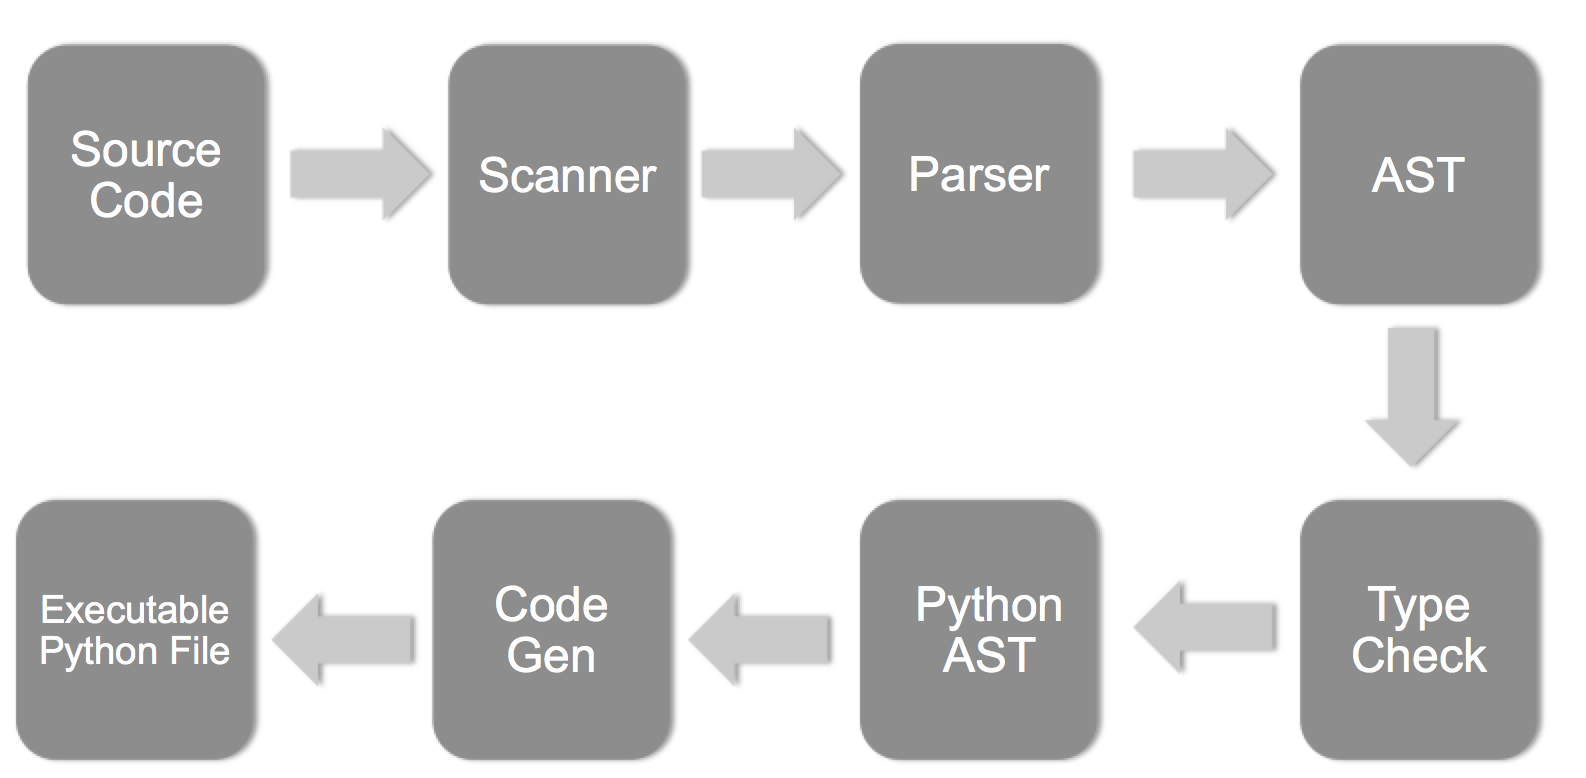
\includegraphics[width=\textwidth]{pipeline}
\caption{Pipeline}
\end{figure}

\subsubsection{Scanner (Guitang, Chenzhe, Liang)}
\noindent Because LFLA doesn't support string and char types. So Scanner.mll only needs to accept identifiers, literals, operators, reserved words, etc. Scanner.mll also throw exception when meeting syntax error and give out which line of code goes wrong.

\subsubsection{Parser (Zhiyuan, Guitang) }
\noindent Parser.mll takes in the tokens generated by Scanner and generate AST based on the grammar rules provided. 

\subsubsection{Type Checker (Zhiyuan, Chenzhe)}
\noindent During translating AST to Python AST, program informations are all stored in translation environment, a data structure containing several symbol tables. When doing type checking, it first looks for type imformation of a expression from symbol tables, and do pattern matching based on our type restrictions.

\subsubsection{Code Generator (Zhiyuan, Guitang, Liang)}
\noindent Taking in python AST, compile.ml translate it into python code. One thing need to pay attention is the indentation in the python code.

\subsection{Python Library}
\noindent Python library is an important part for LFLA. It implements some basic mathematical classes and functionalities. It uses python numpy package as a main tool.

\subsubsection{Basic Classes (Chenzhe, Guitang)}
\noindent VecSpace.py, InSpace.py and AffSpace.py implements three major data types vector space, inner product space and affine space and their related functions. For VecSpace.py, it stores a list vectors internally as a basis in vector space. For InSpace, it owns a list of vectors and a matrix internally. For AffSpace, it has a vector and a vector space internally. They all provide simple interfaces that can be easily used when we generate python code.

\subsubsection{Builtin Functions (ChenZhe, Guitang)}
\noindent Core.py implements main builtin functions such as rank, trace, ceil, floor, etc, which are provided in LFLA. 


\section{Test Plan}
\subsection{Source to Target}
\noindent Two representative source language programs are shown here, along with the corresponding target program for each. \\

\noindent Source Program 1: \\
\begin{lstlisting}
function main()
{   
vector v1 = [1,2,3];
vector v2 = [2,3,4];
vector v3 = [3,5,7];
vecspace vs1 = L(v1, v2);
vecspace vs2 = L(v1, v2, v3);
vecspace vs3 = L();
vector vecs[3] = {v1,v2,v3};
vecspace vs4 = L(vecs);
print(basis(vs1));
print(basis(vs2));
print(basis(vs3));
print(basis(vs4));
}
\end{lstlisting}

\noindent Target Program 1: \\
\begin{lstlisting}
#!/usr/bin/python
import sys
sys.path.append('./lib')
from InSpace import *
from AffSpace import *
from Core import * 

def main() :
v1=np.array([1,2,3])
v2=np.array([2,3,4])
v3=np.array([3,5,7])
vs1=VecSpace([v1,v2])
vs2=VecSpace([v1,v2,v3])
vs3=VecSpace([])
vecs=[v1,v2,v3]
vs4=VecSpace(vecs)
print(vs1.basis())
print(vs2.basis())
print(vs3.basis())
print(vs4.basis())

main()	
\end{lstlisting}

$ $\\
\noindent Source Program 2: \\
\begin{lstlisting}

function main()
{
matrix a = [ 1,2;3,4;];
matrix b = [1,1,1;1,1,1;];
matrix c = a *b;
print(c);
}
\end{lstlisting}
\noindent Target Program 2: \\
\begin{lstlisting}
#!/usr/bin/python
import sys
sys.path.append('./lib')
from InSpace import *
from AffSpace import *
from Core import * 

def main() :
a=np.matrix(((1,2),(3,4)))
b=np.matrix(((1,1,1),(1,1,1)))
c=a * b
print(c)

main()
\end{lstlisting}

\noindent Source Program 3: \\
\begin{lstlisting}
function main()
{
vector v1 = [1,0,0];
vector v2 = [0,1,0];
vector v3 = [0,0,1];

matrix mat = [1,0,0;0,1,0;0,0,1;];
vector vecs[3] = {v1, v2, v3};
inspace ins = inspace(vecs, mat);  
print(dim(ins));		
}
\end{lstlisting}

\noindent Target Program 3: \\
\begin{lstlisting}
#!/usr/bin/python
import sys
sys.path.append('./lib')
from InSpace import *
from AffSpace import *
from Core import * 

def main() :
v1=np.array([1,0,0])
v2=np.array([0,1,0])
v3=np.array([0,0,1])
mat=np.matrix(((1,0,0),(0,1,0),(0,0,1)))
vecs=[v1,v2,v3]
ins=InSpace(vecs,mat)
print(ins.dim())

main()

\end{lstlisting}


\subsection{Test Suites}
\noindent Several testing strategies and techniques are implemented to achieve the validness and robustness of the LFLA language. Test suites includes positive and negative testing, unit testing and integration testing, white-box and black-box testing, regression testing, and automation testing.\\

\noindent Our tests can be divided into two categories - positive tests and negative ones. Positive tests are designed for valid assertions of statements, which should compile and run successfully, while negative tests aim to detect invalid code, and are expected to fail. Furthermore, both white-box and black-box testing are applied to test the LFLA language. We found that the white-box testing is efficient in finding errors and problems. In the meantime, the black-box testing is good complementary to the white-box testing, and we are able to focus on the functionality of the LFLA language. White-box testing do control flow testing, branch testing, data flow testing, and so forth. \\

\noindent Our testing suites are also conducted in varied levels. We do unit testing on smaller testable units of the LFLA language. Unit testing can catch the bugs early on before any integration, and integration testing is carried out to examine the integrity of the whole system. \\

\noindent Regression testing is the most beneficial testing technique in the whole project. Along with the ongoing changes in the compiler, we recycled our previously established completed tests to check whether the fixed faults have re-emerged. We tried to keep up with the good coding practice. Since it is inefficient to run regression testing manually, we introduce automation testing into our testing suits. With the help of automated testing, we are able to run the code against the tests regularly. We also intuitively use unit testing on the small testable part of the program, which greatly simply the later-on integration testing. Integration testing are constructed to examine whether the components of the compiler.

\subsubsection{Testing Cases}
\noindent Testing cases are written to test the syntax, semantics, and functionality of the LFLA language. Testing cases can start from the very small pieces to the more complete ones. Testing cases aim to test the LFLA language according to the specifications and the Language Reference Manual. Testing cases cover the identifiers, keywords, statements and blocks, control flows, data types, arrays, built-in functions, comments, operators, variable, as well as function declarations and definitions.

\subsubsection{Automation Testing}
\noindent We have about sixty testing cases. Automation becomes necessary as the project is moving forward. At the beginning, we found the automation testing will streamline our workflow of testing. With the test-driven process in mind, we follows the sequences in its life cycle. We create new tests for new or modified features of our language. Then we run all the tests to check if they are working. Next, if the tests fail, we focus on fix the code to pass the tests, and if the tests pass, we repeat the process from the start. We rely heavily on regression testing, and automated testing enable to automate the repeated tasks on previously completed tests.

\subsubsection{Test Roles}
\noindent Jin Liang designed test cases, and reported bugs to the member responsible for the code (Zhiyuan Guo or ChenZhe Qian), who would in turn find and solve the reported error. Guitang Lan created the testing infrastructure.


\section{Lessons Learned}

\subsection{Chenzhe Qian}
\noindent I learned several things from this project. First, to have a holistic view of the whole project is the key. Such view can offer a great and efficient management to complete the project. Though no one can know everything before head, it is good to approximate the difficulty of each components. Second, knowing the capability of each team member is significant. As a team, we need to assign various tasks to different team members. If we can make good use of everyone, it affects a lot. Last, we need act as a team. Even in a small team of size four, team work is way more powerful than individual work if we can act like a whole.

\subsection{Guitian Lan}
\noindent First, about team management : for a small team,  hierachical structure is a better choice for team management. Democracy will only make the project never end. Also, communication and compromise are key to efficient team; Second, about meeting: it is better to make a detail plan before weekly meeting, otherwise it is easy to become a chit chat. Finally, about coding:  it is difficult to code the same file with others. Coding is a very private thing. It is better to divide the program into several modules, so that each member works on one module by their own.   \\
Advice: Start the project at the first day of class. It is never too earlier to stat the project. 
\subsection{Jin Liang}
\noindent Starting early is the key. Ocaml is hard to get started. Compiler is cool. LFLA Team is A-Team.
\subsection{Zhiyuan Guo}
\noindent This course is one that theory and practical are tightly combined. Only read the text book will make everything too abstract to understand. So getting hand dirty and code our own compiler is a perfect way to learn this course. It will help you understand the theory more deeply. For the project management, it is difficult to get a clear path at the beginning of the project. So it will make it a little difficult to allocate tasks to each one clearly. It delay the project process at some level. Team work is important in future, I learned a lot about it from this project.
%----------------------------------------------------------------------

\section{Appendix}

\begin{lstlisting}[style=appendix, caption=scanner.mly]
{ 
open Lexing
open Parser 
(* 
* update line number in the context 
* *)
let next_line lexbuf =
let pos = lexbuf.lex_curr_p in
lexbuf.lex_curr_p <-
{ pos with pos_bol = lexbuf.lex_curr_pos;
pos_lnum = pos.pos_lnum+1
}
}

let Exp = 'e'('+'|'-')?['0'-'9']+

rule token = parse 
[' ' '\t' ]            { token lexbuf }
| ['\r' '\n']| "\r\n"   { next_line lexbuf; token lexbuf }
| "###"                 { comment lexbuf }
| '#'                   { line_comment lexbuf }
(* constructor key words and built-in functions*)
| 'L'       { VSCONST }
| "dim"     { DIM }
| "size"    { SIZE }
| "basis"   { BASIS }
| "print"   { PRINT }
| "rank"    { RANK }
| "trace"   { TRACE }
| "image"   { IMAGE }
| "eigenValue" { EVALUE }
| "ceil"    { CEIL }
| "floor"   { FLOOR }
| "sqrt"    { SQRT }
| "solve"   { SOLVE }

(* several kinds of delimiters *)
| '{'   { LBRACE }
| '}'   { RBRACE }
| '['   { LBRACK }
| ']'   { RBRACK }
| '('   { LPAREN }
| ')'   { RPAREN }
| ';'   { SEMI  }
| ','   { COMMA }
| ':'   { COLON }
| '='   { ASSIGN }
| "[["  { LLBRACK }
| "]]"  { RRBRACK }
| "<<"  { LIN }
| ">>"  { RIN }
(* logical operators *)
| "&&"  { AND }
| "||"  { OR }
(* additive operators *)
| "+"   { PLUS }
| "-"   { MINUS }
| "+."  { PLUS_DOT }
| "-."  { MINUS_DOT }
(* multiplicative operators *)
| '*'   { TIMES }
| '/'   { DIVIDE }
| "*."  { TIMES_DOT }
| "/."  { DIVIDE_DOT }
(* unary operator *)
| '\''  { TRANSPOSE }
| '@'   { BELONGS }
| '&'   { ACTION }
(* comparation operators *)
| '<'   { LT }
| "<="  { LEQ }
| '>'   { GT }
| ">="  { GEQ }
| "=="  { EQ }
| "!="  { NEQ }
(* type identifier *)
| "var"         { VAR }
| "vector"      { VECTOR }
| "vecspace"    { VECSPACE }
| "matrix"      { MATRIX }
| "inspace"     { INSPACE }
| "affspace"    { AFFSPACE }
(* control flow statements *)
| "while"   { WHILE }
| "for"     { FOR }
| "if"      { IF }
| "else"    { ELSE }
| "break"   { BREAK }
| "continue"{ CONTINUE }
| "return"  { RETURN }
(* function declaration *)
| "function"    { FUNCTION }
(* Literal and identifers *)
| ['0'-'9']+ | ('.'['0'-'9']+Exp? 
| ['0'-'9']+ ('.'['0'-'9']*Exp? | Exp))
				as num  { LITERAL(num) }
| ['a'-'z' 'A'-'Z']['a'-'z' 'A'-'Z' '0'-'9' '_']* 
				as id { ID(id) }
| eof       { EOF }
| _ as c 
	{ raise (Failure("illegal character "^Char.escaped c))}

and comment = parse
"###"      { token lexbuf }
| _         { comment lexbuf }

and line_comment = parse
['\n' '\r']   { token lexbuf }
| _             { line_comment lexbuf }
\end{lstlisting}

\begin{lstlisting}[style=appendix, caption=parser.mly]
%{  
    open Ast 
    open Lexing
    open Parsing 

    exception ParseErr of string

    let error msg start finish  = 
        Printf.sprintf "(line %d: char %d..%d): %s" start.pos_lnum 
            (start.pos_cnum -start.pos_bol) (finish.pos_cnum - finish.pos_bol) msg
   
%}

%token VSCONST PRINT DIM SIZE BASIS RANK TRACE IMAGE EVALUE CEIL FLOOR SQRT SOLVE 
%token LBRACE RBRACE LBRACK RBRACK LLBRACK RRBRACK LIN RIN LPAREN RPAREN COLON SEMI COMMA
%token AND OR  
%token PLUS MINUS PLUS_DOT MINUS_DOT 
%token TIMES DIVIDE TIMES_DOT DIVIDE_DOT 
%token ASSIGN
%token TRANSPOSE BELONGS ACTION
%token LT LEQ GT GEQ EQ NEQ 
%token VAR VECTOR VECSPACE MATRIX INSPACE AFFSPACE
%token WHILE FOR IF ELSE BREAK CONTINUE RETURN FUNCTION
%token <string> LITERAL
%token <string> ID
%token EOF

%nonassoc NOELSE
%nonassoc ELSE
%right ASSIGN
%left LBRACK RBRACK
%left LT LEQ GT GEQ EQ NEQ
%left PLUS MINUS PLUS_DOT MINUS_DOT
%left TIMES DIVIDE TIMES_DOT DIVIDE_DOT
%left AND OR
%left TRANSPOSE BELONGS ACTION

%start program
%type<Ast.program> program

%%

program:
    programs EOF { List.rev $1 }

programs :
    /* nothing */                   { [] }
    | programs funtion_declaration  { Function($2)::$1 }
    | programs global_normal_declaration   { Variable($2)::$1 } 
    | error     
        { raise ( ParseErr (error "syntax error" (Parsing.symbol_start_pos ()) 
        (Parsing.symbol_end_pos ()))) }
funtion_declaration :
    FUNCTION ID LPAREN parameter_list_opt RPAREN LBRACE statement_list  RBRACE { 
        {   fname=$2; 
            params=$4; 
            body= List.rev $7;
            ret_type = Unit } }

parameter_list_opt :
    /* nothing */       { [] }
    | parameter_list    { List.rev $1 }

parameter_list :
    primitive_type ID                                           
        { [ Lvardecl({vname = $2; value = Notknown; data_type = $1; pos = let pos_start = Parsing.symbol_start_pos () in pos_start.pos_lnum })] }
    | primitive_type LBRACK RBRACK ID                           
        { [ Larraydecl({ aname = $4; elements = []; data_type = array_type $1; length = max_int; pos = let pos_start = Parsing.symbol_start_pos () in pos_start.pos_lnum})] } 
    | parameter_list COMMA primitive_type ID                    
        { Lvardecl({vname = $4; value = Notknown; data_type = $3; pos = let pos_start = Parsing.symbol_start_pos () in pos_start.pos_lnum})::$1 }
    | parameter_list COMMA primitive_type ID LBRACK RBRACK      
        { Larraydecl({aname = $4; elements = []; data_type = array_type $3; length = max_int; pos = let pos_start = Parsing.symbol_start_pos () in pos_start.pos_lnum})::$1 }
    | error { raise ( ParseErr (error "syntax error" (Parsing.symbol_start_pos ()) (Parsing.symbol_end_pos ()))) }

local_normal_declaration :
    local_normal_declaration_expression SEMI { $1 }

local_normal_declaration_expression :
    variable_declaration_expression { Lvardecl($1) }
    | array_declaration_expression  { Larraydecl($1) }

global_normal_declaration :
    global_normal_declaration_expression SEMI { $1 }

global_normal_declaration_expression :
    variable_declaration_expression { Gvardecl($1) }
    | array_declaration_expression  { Garraydecl($1) }

variable_declaration_expression :
    var_declaration_expression          { $1 }
    | vector_declaration_expression     { $1 }  
    | matrix_declaration_expression     { $1 }
    | vecspace_declaration_expression   { $1 }
    | inspace_declaration_expression    { $1 }
    | affspace_declaration_expression   { $1 }

var_declaration_expression :
    VAR ID                      
        { 
            {vname = $2; value = Notknown; data_type = Var; 
            pos = let pos_start = Parsing.symbol_start_pos () in pos_start.pos_lnum } 
        }
   /* | VAR ID ASSIGN LITERAL     { Vardecl({vname = $2; value = VValue($4); data_type = Var }) }  expression contains LITERAL   */ 
    | VAR ID ASSIGN expression  
        { 
            {vname = $2; value = Expression(Var,$4); data_type = Var; 
            pos = let pos_start = Parsing.symbol_start_pos () in pos_start.pos_lnum } 
        }

vector_declaration_expression :
    VECTOR ID   
        { 
            {vname = $2; value = Notknown; data_type = Vector; 
            pos = let pos_start = Parsing.symbol_start_pos () in pos_start.pos_lnum } 
        }
   /* | VECTOR ID ASSIGN LBRACK vector_elements_list_opt RBRACK 
        { 
            {vname = $2; value = VecValue($5); data_type = Vector; 
            pos = let pos_start = Parsing.symbol_start_pos () in pos_start.pos_lnum } 
        }*/
    | VECTOR ID ASSIGN expression
        { 
            {vname = $2; value = Expression(Vector, $4); data_type = Vector; 
            pos = let pos_start = Parsing.symbol_start_pos () in pos_start.pos_lnum } 
        }

vector_elements_list_opt :
    /* nothing */           { [] }
    | vector_elements_list  { List.rev $1 }

vector_elements_list :
    LITERAL                                 { [$1] }
    | MINUS LITERAL                           { [String.concat "" ["-";$2]] }
    | vector_elements_list COMMA LITERAL    { $3::$1 }
    | vector_elements_list COMMA MINUS LITERAL  { (String.concat "" ["-";$4])::$1 }
    | error 
        { raise ( ParseErr (error "syntax error" (Parsing.symbol_start_pos ()) (Parsing.symbol_end_pos ()))) }

matrix_declaration_expression :
    MATRIX ID   
        { 
            {vname = $2; value = Notknown; data_type = Matrix; 
            pos = let pos_start = Parsing.symbol_start_pos () in pos_start.pos_lnum } 
        }
   /* | MATRIX ID ASSIGN LBRACK matrix_elements_list RBRACK 
        { 
            {vname = $2; value = MatValue($5); data_type = Matrix; 
            pos = let pos_start = Parsing.symbol_start_pos () in pos_start.pos_lnum } 
        } */
    | MATRIX ID ASSIGN expression
        { 
            {vname = $2; value = Expression(Matrix, $4); data_type = Matrix; 
            pos = let pos_start = Parsing.symbol_start_pos () in pos_start.pos_lnum } 
        }


matrix_elements_list :
    vector_elements_list SEMI       { [List.rev $1] }
    | vector_elements_list SEMI matrix_elements_list { (List.rev $1)::$3 }


vecspace_declaration_expression :
    VECSPACE ID 
        { 
            {vname = $2; value = Notknown; data_type = VecSpace; 
            pos = let pos_start = Parsing.symbol_start_pos () in pos_start.pos_lnum }
        }
    | VECSPACE ID ASSIGN expression
        {
            {vname = $2; value = Expression(VecSpace, $4); data_type = VecSpace;
            pos = let pos_start = Parsing.symbol_start_pos () in pos_start.pos_lnum }
        }


inspace_declaration_expression :
    INSPACE ID  
        { 
            {vname = $2; value = Notknown; data_type = InSpace; 
            pos = let pos_start = Parsing.symbol_start_pos () in pos_start.pos_lnum } 
        }
    | INSPACE ID ASSIGN INSPACE LPAREN expression COMMA expression RPAREN 
        { 
            {vname = $2; value = InSpValue($6,$8); data_type = InSpace; 
            pos = let pos_start = Parsing.symbol_start_pos () in pos_start.pos_lnum } 
        }

affspace_declaration_expression :
    AFFSPACE ID 
        { 
            {vname = $2; value = Notknown; data_type = AffSpace; 
            pos = let pos_start = Parsing.symbol_start_pos () in pos_start.pos_lnum } 
        }
    | AFFSPACE ID ASSIGN AFFSPACE LPAREN expression COMMA expression RPAREN 
        { 
            {vname = $2; value = AffSpValue($6, $8); data_type = AffSpace; 
            pos = let pos_start = Parsing.symbol_start_pos () in pos_start.pos_lnum } 
        }

array_declaration_expression :
    VAR ID LBRACK LITERAL RBRACK 
        { 
            try { aname = $2; elements = []; data_type = VarArr; length = int_of_string $4; 
            pos = let pos_start = Parsing.symbol_start_pos () in pos_start.pos_lnum} 
            with Failure "int_of_string" -> raise(Failure "not valid array length");
        }
    | VAR ID LBRACK LITERAL RBRACK ASSIGN LBRACE array_elements_list RBRACE 
        { 
            try { aname = $2; elements = (List.rev $8); data_type = VarArr; length = int_of_string $4; 
            pos = let pos_start = Parsing.symbol_start_pos () in pos_start.pos_lnum}
            with Failure "int_of_string" -> raise(Failure "not valid array length");
        }
    | VECTOR ID LBRACK LITERAL RBRACK 
        { 
            try { aname = $2; elements = []; data_type = VectorArr; length = int_of_string $4; 
            pos = let pos_start = Parsing.symbol_start_pos () in pos_start.pos_lnum}
            with Failure "int_of_string" -> raise(Failure "not valid array length");
        }
    | VECTOR ID LBRACK LITERAL RBRACK ASSIGN LBRACE array_elements_list RBRACE 
        { 
            try { aname = $2; elements = (List.rev $8); data_type = VectorArr; length = int_of_string $4; 
            pos = let pos_start = Parsing.symbol_start_pos () in pos_start.pos_lnum}
            with Failure "int_of_string" -> raise(Failure "not valid array length");
        }
    | MATRIX ID LBRACK LITERAL RBRACK 
        { 
            try { aname = $2; elements = []; data_type = MatrixArr; length = int_of_string $4; 
            pos = let pos_start = Parsing.symbol_start_pos () in pos_start.pos_lnum}
            with Failure "int_of_string" -> raise(Failure "not valid array length");
        }
    | MATRIX ID LBRACK LITERAL RBRACK ASSIGN LBRACE array_elements_list RBRACE 
        { 
            try { aname = $2; elements = (List.rev $8); data_type = MatrixArr; length = int_of_string $4; 
            pos = let pos_start = Parsing.symbol_start_pos () in pos_start.pos_lnum}
            with Failure "int_of_string" -> raise(Failure "not valid array length");
        }
    | INSPACE ID LBRACK LITERAL RBRACK 
        { 
            try { aname = $2; elements = []; data_type = InSpaceArr; length = int_of_string $4; 
            pos = let pos_start = Parsing.symbol_start_pos () in pos_start.pos_lnum}
            with Failure "int_of_string" -> raise(Failure "not valid array length");
        }
    | INSPACE ID LBRACK LITERAL RBRACK ASSIGN LBRACE array_elements_list RBRACE 
        { 
            try { aname = $2; elements = (List.rev $8); data_type = InSpaceArr; length = int_of_string $4; 
            pos = let pos_start = Parsing.symbol_start_pos () in pos_start.pos_lnum}
            with Failure "int_of_string" -> raise(Failure "not valid array length");
        }
    | AFFSPACE ID LBRACK LITERAL RBRACK 
        { 
            try { aname = $2; elements = []; data_type = AffSpaceArr; length = int_of_string $4; 
            pos = let pos_start = Parsing.symbol_start_pos () in pos_start.pos_lnum}
            with Failure "int_of_string" -> raise(Failure "not valid array length");
        }
    | AFFSPACE ID LBRACK LITERAL RBRACK ASSIGN LBRACE array_elements_list RBRACE 
        { 
            try { aname = $2; elements = (List.rev $8); data_type = AffSpaceArr; length = int_of_string $4; 
            pos = let pos_start = Parsing.symbol_start_pos () in pos_start.pos_lnum}
            with Failure "int_of_string" -> raise(Failure "not valid array length");
        }
    | VECSPACE ID LBRACK LITERAL RBRACK 
        { 
            try { aname = $2; elements = []; data_type = VecSpaceArr; length = int_of_string $4; 
            pos = let pos_start = Parsing.symbol_start_pos () in pos_start.pos_lnum}
            with Failure "int_of_string" -> raise(Failure "not valid array length");
        }
    | VECSPACE ID LBRACK LITERAL RBRACK ASSIGN LBRACE array_elements_list RBRACE 
        { 
            try { aname = $2; elements = (List.rev $8); data_type = VecSpaceArr; length = int_of_string $4; 
            pos = let pos_start = Parsing.symbol_start_pos () in pos_start.pos_lnum}
            with Failure "int_of_string" -> raise(Failure "not valid array length");
        }

array_elements_list :
    | expression                           { [$1] }
    | array_elements_list COMMA expression { $3::$1 }


statement :
    expression SEMI                 { Expr($1) }
    | RETURN    expression SEMI     { Return($2) }
    | BREAK     SEMI                { Break }
    | CONTINUE  SEMI                { Continue }
    | LBRACE statement_list RBRACE  { Block(List.rev $2) }
    | IF expression LBRACE statement_list RBRACE %prec NOELSE 
                                    { If($2, List.rev $4, []) }
    | IF expression LBRACE statement_list RBRACE ELSE LBRACE statement_list RBRACE 
                                    { If($2, List.rev $4, List.rev $8) }
    | FOR ID ASSIGN expression COLON expression LBRACE statement_list RBRACE 
                                    { For($2, $4, $6,List.rev($8)) } /* TODO: if var is needed here */
    | WHILE expression LBRACE statement_list RBRACE { While($2, List.rev $4) }
    | local_normal_declaration      { Decl($1) }

statement_list :
    /* nothing */ { [] }
    | statement_list statement { $2::$1 }

expression:
    LITERAL                             { Literal($1) }
    | element                           { Id($1) }
    | MINUS LITERAL                     { Literal(String.concat "" ["-";$2]) }
    | expression TRANSPOSE              { Callbuiltin(Transpose, [$1]) }
    | expression PLUS       expression  { Binop($1, Add, $3) }
    | expression MINUS      expression  { Binop($1, Sub, $3) }
    | expression TIMES      expression  { Binop($1, Mult, $3) }
    | expression DIVIDE     expression  { Binop($1, Div, $3) }
    | expression EQ         expression  { Binop($1, Equal, $3) }
    | expression NEQ        expression  { Binop($1, Neq, $3) }
    | expression LT         expression  { Binop($1, Less, $3) }
    | expression LEQ        expression  { Binop($1, Leq, $3) }
    | expression GT         expression  { Binop($1, Greater, $3) }
    | expression GEQ        expression  { Binop($1, Geq, $3) }
    | expression AND        expression  { Binop($1, And, $3) }
    | expression OR         expression  { Binop($1, Or, $3) }
    | expression PLUS_DOT   expression  { Binop($1, Add_Dot, $3) }
    | expression MINUS_DOT  expression  { Binop($1, Sub_Dot, $3) }
    | expression TIMES_DOT  expression  { Binop($1, Mult_Dot, $3) }
    | expression DIVIDE_DOT expression  { Binop($1, Div_Dot, $3) }
    | expression BELONGS    expression  { Callbuiltin(Belongs, [$1;$3]) }
    | expression ACTION     expression  { Callbuiltin(Action, [$1;$3]) }
    | ID     LIN expression  COMMA   expression  RIN     { Callbuiltin(Inpro, [Id(Nid($1));$3;$5]) }
    | LLBRACK   expression  COMMA   expression  RRBRACK { Callbuiltin(LieBracket, [$2;$4]) }   
    | element    ASSIGN  expression                          { Assign($1, $3) }
    | element    ASSIGN  LBRACE array_elements_list RBRACE   { AssignArr($1, $4) } 
    | LBRACK vector_elements_list_opt RBRACK            { ExprValue(VecValue($2)) }
    | LBRACK matrix_elements_list RBRACK                { ExprValue(MatValue($2)) }
    | INSPACE LPAREN expression COMMA expression RPAREN { ExprValue(InSpValue($3, $5)) }
    | AFFSPACE LPAREN expression COMMA expression RPAREN{ ExprValue(AffSpValue($3, $5)) }  
    | VSCONST   LPAREN  arguments_opt  RPAREN           { ExprValue(VecSpValue($3)) }   
    | ID    LPAREN  arguments_opt RPAREN                { Call($1, $3) } 
    | LPAREN    expression  RPAREN                      { $2 }
    | builtin   LPAREN  arguments_opt  RPAREN           { Callbuiltin($1, $3) }

builtin:
    DIM         { Dim }
    | SIZE      { Size }
    | BASIS     { Basis }
    | TRACE     { Trace }
    | RANK      { Rank }
    | IMAGE     { Image }
    | EVALUE    { Evalue }
    | CEIL      { Ceil }
    | FLOOR     { Floor }
    | SQRT      { Sqrt }
    | SOLVE     { Solve }
    | PRINT     { Print }
    | error     { raise ( ParseErr (error "syntax error" (Parsing.symbol_start_pos ()) 
    (Parsing.symbol_end_pos ()))) }

/* normal identifier and array identifier */
element:
    | ID                          { Nid($1) }
    | ID LBRACK LITERAL RBRACK      { Arrayid($1, $3) }
    | ID LBRACK ID      RBRACK      { Arrayid($1, $3) }

arguments_opt:
    /* nothing */   { [] }
  | arguments_list  { List.rev $1 }

arguments_list:
    expression        { [$1] }       
  | arguments_list COMMA expression { $3::$1 } 

primitive_type:
    VAR         { Var }
    | VECTOR    { Vector }
    | VECSPACE  { VecSpace }
    | MATRIX    { Matrix }
    | INSPACE   { InSpace }
    | AFFSPACE  { AffSpace }
    | error     { raise ( ParseErr (error "syntax error" (Parsing.symbol_start_pos ()) 
    (Parsing.symbol_end_pos ()))) }
\end{lstlisting}

\begin{lstlisting}[style=appendix, caption=ast.ml]
(* operators *)
type op = Add | Sub | Mult | Div | Add_Dot | Sub_Dot | Mult_Dot 
        | Div_Dot | Equal | Neq | Less | Leq | Greater | Geq
        | And | Or  
(* 
 * element, normal id or 
 * array id with index 
 * *)
type elem = 
  | Nid of string  (* normal identifier *)
  | Arrayid of string * string (* array identifier *)

(* builtin functions *)
type builtin_func = 
    Sqrt
  | Ceil
  | Floor
  | Dim
  | Size
  | Basis
  | Image
  | Rank
  | Trace
  | Evalue
  | Solve
  | Belongs
  | LieBracket
  | Inpro
  | Transpose
  | Print
  | Action

(* primitive types, seperate 
 * noraml types and array types 
 * *)
type prim_type = 
    Var
  | Vector
  | Matrix
  | VecSpace
  | InSpace
  | AffSpace
  | VarArr
  | VectorArr
  | MatrixArr
  | VecSpaceArr
  | InSpaceArr
  | AffSpaceArr
  | Unit

(* expressions 
 * *)
type expr =
    Literal of string
  | Id of elem
  | Binop of expr * op * expr
  | Assign of elem * expr
  | AssignArr of elem * expr list
  | Call of string * expr list
  | Callbuiltin of builtin_func * expr list
  | ExprValue of prim_value
  | Noexpr

(*  value of primitive types *)
and prim_value = 
    VValue of string
  | VecValue of string list
  | MatValue of string list list
  | VecSpValue of expr list
  | InSpValue of expr * expr
  | AffSpValue of expr * expr
  | Expression of prim_type * expr
  | Notknown

(* variable declaration
 * vname : name of variable
 * value : value of variable
 * data_type : type of variable
 * pos : position in original code(not used)
 * *)
type var_decl = {
    vname : string;
    value : prim_value;
    data_type : prim_type;
    pos : int;
}

(* array declaration
 * aname : name of array identifier
 * elements : expression list represents the elements of array
 * length : length of the array
 * data_type : type of variable
 * pos : position in original code(not used)
 * *)
type array_decl = {
    aname : string;
    elements : expr list;
    data_type : prim_type;
    mutable length : int;
    pos : int;
}

(* combine variable declarations and array declarations 
 * only represent global declaration
 * *)
type gNormal_decl = 
    Gvardecl of var_decl
  | Garraydecl of array_decl

(* combine variable declarations and array declarations 
 * only represent local declaration
 * *)
type lNormal_decl = 
    Lvardecl of var_decl
  | Larraydecl of array_decl 

(* statements *)
type stmt =
    Block of stmt list
  | Expr of expr
  | Return of expr
  | If of expr * stmt list * stmt list
  | For of string * expr * expr * stmt list
  | While of expr * stmt list
  | Continue
  | Break
  | Decl of lNormal_decl 

(* function declaration 
 * fname : name of function
 * params : list of local normal declarations
 * body : main part of function, a list of statments
 * ret_type : return type of function
 *)
type func_decl = {
    fname : string;
    params : lNormal_decl list;
    body : stmt list;
    ret_type : prim_type;
}

(* combine gloval variable declaration and funciton declaration *)
type program_stmt =
    Variable of gNormal_decl
  | Function of func_decl

type program = program_stmt list

(* input : prim_type
 * output : prim_type
 * get the real data type if it is a array type 
 * otherwise remain same
 * *)
let real_type = function
    Var -> Var
    | Vector -> Vector
    | Matrix -> Matrix
    | VecSpace -> VecSpace
    | InSpace -> InSpace
    | AffSpace -> AffSpace
    | VarArr -> Var
    | VectorArr -> Vector
    | MatrixArr -> Matrix
    | VecSpaceArr -> VecSpace
    | InSpaceArr -> InSpace
    | AffSpaceArr -> AffSpace
    | Unit -> Unit 

(* input : prim_type
 * output : prim_type
 * get the array data if it is a normal type
 * otherwise remain same
 * *)
let array_type = function
    Var -> VarArr
    | Vector -> VectorArr
    | Matrix -> MatrixArr
    | VecSpace -> VecSpaceArr
    | InSpace -> InSpaceArr
    | AffSpace -> AffSpaceArr
    | VarArr -> VarArr
    | VectorArr -> VectorArr
    | MatrixArr -> MatrixArr
    | VecSpaceArr -> VecSpaceArr
    | InSpaceArr -> InSpaceArr
    | AffSpaceArr -> AffSpaceArr
    | Unit -> Unit
\end{lstlisting}

\begin{lstlisting}[style=appendix, caption=translate.ml]
open Ast
open Past
open Check
open Translate_env

(* module StringMap = Map.Make(String) *)

(* input : ast operator
 * output : past operator
 * translate ast operator to python ast operator 
 * *)
let translate_op = function
    Add -> Padd
    | Sub -> Psub
    | Mult -> Pmult
    | Div -> Pdiv
    | Add_Dot -> Padd_Dot
    | Sub_Dot -> Psub_Dot
    | Mult_Dot -> Pmult_Dot
    | Div_Dot -> Pdiv_Dot
    | Equal -> Pequal
    | Neq -> Pneq
    | Less -> Pless
    | Leq -> Pleq
    | Greater -> Pgreater
    | Geq -> Pgeq
    | And -> Pand
    | Or -> Por

(* input : ast operator
 * output : past operator
 * translate ast prim type to python ast prim type *)
let translate_prim_type = function
    Var -> P_var
    | Vector -> P_vector
    | Matrix -> P_matrix
    | VecSpace -> P_vecSpace
    | InSpace -> P_inSpace
    | AffSpace -> P_affSpace
    | VarArr -> P_varArr
    | VectorArr -> P_vectorArr
    | MatrixArr -> P_matrixArr
    | VecSpaceArr -> P_vecSpaceArr
    | InSpaceArr -> P_inSpaceArr
    | AffSpaceArr -> P_affSpaceArr
    | Unit -> P_unit

(* input: ast element
 * output: past element
 * translate ast element to python ast element, and
 * check symbol tables, throw exception if they are not defined
 * *)
let translate_elem env = function
    | Nid(s) -> 
        if is_defined_var s env then
            P_nid(s)
        else raise(Failure ("undeclared identifier " ^ s))
    | Arrayid(s1, s2) -> 
        if is_defined_var s1 env then
            P_arrayid(s1, s2)
        else raise(Failure ("undeclared identifier " ^ s1))

(* input: env->translate_env and ast expression list
 * output: past expression list and updated env
 * traverse_exprs works to translate a list of expression 
 * *)
let rec traverse_exprs env = function
    [] -> [], env
    | hd::tl -> 
        let pE, env = translate_expr env hd in
        let pTl, env = traverse_exprs env tl in
        pE::pTl, env
(* input: ast expression and translate environment
 * output: past expression and updated environment
 * translate ast expr to python ast expr and do some basic checks
 * *)
and translate_expr env = function 
    Literal(l) -> (P_literal(l), env)
    | Id(el) -> 
        (P_id(translate_elem env el), env)
    | Binop(e1, o, e2) -> 
        let (pE1, env) = translate_expr env e1 in
        let pO = translate_op o in
        let (pE2, env) = translate_expr env e2 in
        (match (type_of env e1, o, type_of env e2) with
            Matrix, Mult_Dot, Matrix -> (P_matrixMul(pE1, pE2), env)
            |_,_,_ -> (P_binop(pE1, pO, pE2), env))
    | Assign(el, e) -> (* TODO: update the id in symbol table *) 
            if not (is_defined_element el env) then
               raise(Failure("undefined identifier"))
            else
                let pE, env = translate_expr env e in
                let pEl = translate_elem env el in    
                    P_assign(pEl, pE), env
    | AssignArr(el, e) -> 
            if not (is_defined_element el env) then
                raise(Failure("undefined identifier"))
            else
                let pE, env = traverse_exprs env e in
                let pEl = translate_elem env el in    
                    P_assignArr(pEl, pE), env
    | Call(f, el) -> 
            if not (is_func f env) then
                raise(Failure("undefined funciton"))
            else
                let pE, env = traverse_exprs env el in
                    (P_call(f, pE), env)
    | Callbuiltin(f, el) -> (*TODO: check the builtin function types *) 
            if (List.length el) == 0 then
                raise(Failure("wrong arguments in builtin funciton"))
            else
            let pElist, env = traverse_exprs env el in
            (match f with
            | Sqrt -> P_sqrt(List.hd pElist), env
            | Ceil -> P_ceil(List.hd pElist), env
            | Floor -> P_floor(List.hd pElist), env 
            | Dim -> 
                    let pE = List.hd pElist in 
                    let typ = type_of env (List.hd el)in
                    P_dim( translate_prim_type typ, pE), env
            | Size -> P_size(List.hd pElist), env
            | Basis -> P_basis(List.hd pElist), env
            | Image -> P_image(List.hd pElist), env
            | Rank -> P_rank(List.hd pElist), env
            | Trace -> P_trace(List.hd pElist), env
            | Evalue -> P_evalue(List.hd pElist), env
            | Solve -> 
                    if (List.length pElist) <> 2 then
                        raise(Failure("wrong arguments in builtin function"))
                    else P_solve(List.hd pElist, List.nth pElist 1), env
            | Belongs -> 
                    if (List.length pElist) <> 2 then
                        raise(Failure("wrong arguments in builtin funciton"))
                    else P_belongs(List.hd pElist, List.nth pElist 1), env
            | LieBracket ->
                    if (List.length pElist) <> 2 then
                        raise(Failure("wrong arguments in builtin function"))
                    else P_lieBracket(List.hd pElist, List.nth pElist 1), env
            | Inpro ->
                    if (List.length pElist) <> 3 then
                        raise(Failure("wrong arguments in builtin function"))
                    else P_inpro(List.hd pElist, List.nth pElist 1, List.nth pElist 2), env
            | Transpose -> P_transpose(List.hd pElist), env
            | Action -> 
                    if (List.length pElist) <> 2 then
                        raise(Failure("wrong arguments in builtin function"))
                    else P_action(List.hd pElist, List.nth pElist 1), env
            | Print -> P_print(List.hd pElist), env
            )  
    | ExprValue(v) -> 
        let pV, env = translate_prim_value env v in
            P_exprValue(pV), env
    | Noexpr -> P_noexpr, env

(* input: ast prim_value and translate environment
 * output: past prim_value and updated environment
 * translate ast prim_value to past prim_value
 * do type checking during translation
 * *)
and translate_prim_value env = function
    VValue(s) -> P_Value(s), env
    | VecValue(s) -> P_VecValue(s), env 
    | MatValue(s) -> P_MatValue(s), env
    | VecSpValue(eList) -> 
            let pEList,env = traverse_exprs env eList in
                if check_list env Vector eList then
                        P_VecSpValue(pEList), env
                else if (List.length eList == 1) then
                    if check_list env VectorArr eList then
                        P_VecSpValueArr(pEList), env
                    else
                        raise(Failure("in vsconst fail in type checking"))
                else
                    raise(Failure("in vsconst fail in type checking"))
    | InSpValue(e1, e2) -> 
            let pE1, env = translate_expr env e1 in
            let pE2, env = translate_expr env e2 in
                let typ1 = type_of env e1 in
                let typ2 = type_of env e2 in
                    if typ1 <> VectorArr || typ2 <> Matrix then
                        raise(Failure("in InSpace construct fail in type checking"))
                    else    
                        P_InSpValue(pE1, pE2), env            
    | AffSpValue(e1, e2) -> 
            let pE1, env = translate_expr env e1 in
            let pE2, env = translate_expr env e2 in
                let typ1 = type_of env e1 in
                let typ2 = type_of env e2 in
                    if typ1 <> Vector || typ2 <> VecSpace then
                        raise(Failure("in AffSpace construct fail in type checking"))
                    else
                        P_AffSpValue(pE1, pE2), env 
    | Expression(typ, e) -> 
            let pExpr, env = translate_expr env e in
                let typ' = type_of env e in
                    if typ' <> typ then
                        raise(Failure("in construct fail in type checking"))
                    else
                        P_Expression(pExpr), env
    | Notknown -> P_Notknown, env
   
(* input: ast local declaration and translate environment
 * output: past local declaration and updated environment
 * translate local variables to python ast variables *)
let translate_local_normal_decl env local_var = 
    match local_var with
    Lvardecl(v) ->
        let pValue, env = translate_prim_value env v.value in
        let p_var =  {  p_vname = v.vname; 
                        p_value = pValue; 
                        p_data_type = translate_prim_type v.data_type; 
                        p_pos = v.pos   } 
        in
        let vars' = 
            if (not (is_defined_var v.vname env)) then
                StringMap.add v.vname local_var env.scope.vars
            else
                raise(Failure("Already defined variable  " ^ v.vname))
        in
        let scope' = { env.scope with vars = vars' } in
        let env' = { env with scope = scope' } in
        P_Vardecl(p_var), env'
           
    | Larraydecl(a) -> 
        let length = List.length a.elements in
        if length <> 0 && length <> a.length then  (* length = 0 occurs only when a is function param *)
            raise(Failure("array length not match"))
        else
        let pExprs, env = traverse_exprs env a.elements in
        if not (check_list env (real_type a.data_type) a.elements) then (* check if array elements have right type *)
            raise(Failure("array elements have wrong type"))
        else
        let p_array = { p_aname = a.aname; 
                        p_elements = pExprs;
                        p_data_type = translate_prim_type a.data_type; 
                        p_length = a.length;
                        p_pos = a.pos   } 
        in
        let vars' = 
            if (not (is_defined_var a.aname env)) then
                StringMap.add a.aname local_var env.scope.vars
            else
                raise(Failure("Already defined variable  " ^ a.aname))
        in
        let scope' = { env.scope with vars = vars' } in
        let env' = { env with scope = scope' } in
        P_Arraydecl(p_array), env'

(* input: ast global declaration and translate environment
 * output: past global declaration and updated environment
 * translate global variables to python ast variables *)
let translate_global_normal_decl env global_var = 
    match global_var with
    Gvardecl(v) ->
        let pValue, env = translate_prim_value env v.value 
        in                                              (* for global variable, local_vars table is empty *)
        let p_var =  {  p_vname = v.vname; 
                        p_value = pValue; 
                        p_data_type = translate_prim_type v.data_type; 
                        p_pos = v.pos   } 
        in
        let global_vars' = 
            if (not (is_global_var v.vname env)) then
                StringMap.add v.vname global_var env.global_vars
            else
                raise(Failure("Already defined variable " ^ v.vname))
        in
        let env' = { env with global_vars = global_vars' } in 
        P_Vardecl(p_var), env'
           
    | Garraydecl(a) -> 
        let length = List.length a.elements in
        if length <> 0 && length <> a.length then  (* length = 0 occurs only when a is a function param *)
            raise(Failure("array length not match"))
        else
        let pExprs, env = traverse_exprs env a.elements 
        in
        if not (check_list env (real_type a.data_type) a.elements) then  (* check for each element if it has right type *)
           raise(Failure("array elements have wrong type"))
        else                                                    (* for global array, local_vars table is empty*)
        let p_array = { p_aname = a.aname; 
                        p_elements = pExprs;
                        p_data_type = translate_prim_type a.data_type; 
                        p_length = a.length;
                        p_pos = a.pos} 
        in
            let global_vars' = 
                if (not (is_global_var a.aname env)) then
                    StringMap.add a.aname global_var env.global_vars
                else
                    raise(Failure("Already defined variable " ^ a.aname))
            in
            let env' = { env with global_vars = global_vars' } in
            P_Arraydecl(p_array), env'

(* input: return expression list, 
 *        function body statements,
 *        translate environment
 * output: return expression list
 * collect all return expressions in function
 * *)
let rec find_return_exprs env ret_exprs body= 
    match body with
        [] -> ret_exprs
        | hd::tl ->
                (match hd with 
                    Return(e) -> 
                        let ret_exprs' = e::ret_exprs in
                            find_return_exprs env ret_exprs' tl
                    | Block(stmts) -> 
                            let ret_exprs1 = find_return_exprs env ret_exprs stmts in
                            find_return_exprs env ret_exprs1 tl
                    | Expr(e) -> 
                            find_return_exprs env ret_exprs tl
                    | If(e, s1, s2) ->
                            let ret_exprs1 = find_return_exprs env ret_exprs s1 in
                            let ret_exprs2 = find_return_exprs env ret_exprs1 s2 in
                                find_return_exprs env ret_exprs2 tl
                    | While(e, s) ->
                            let ret_exprs1 = find_return_exprs env ret_exprs s in
                                find_return_exprs env ret_exprs1 tl
                    | For(v, e1, e2, s) ->
                            let ret_exprs1 = find_return_exprs env ret_exprs s in
                                find_return_exprs env ret_exprs1 tl
                    | Continue -> 
                            find_return_exprs env ret_exprs tl
                    | Break ->
                            find_return_exprs env ret_exprs tl
                    | Decl(l) ->
                            find_return_exprs env ret_exprs tl  
                     
                )
(* input: return expression list,
 *        translate environment
 * output: prim_type 
 * find the return type and check the consistancy
 * *)
let find_return_type env ret_exprs =
    if (List.length ret_exprs) == 0 then
        Unit
    else
    let expr = List.hd ret_exprs in
    let ret_typ = type_of env expr in
        if (check_list env ret_typ ret_exprs) then 
            ret_typ
        else
            raise(Failure "function return type don't match")

(* input: ast statments list
 *        translate environment
 * output: past statements list
 * translate a list of statements 
 * *)
let rec traverse_stmts env = function
    [] -> [], env
    | hd::tl -> 
        let pStmt, env = translate_stmt env hd in
        let pTl, env = traverse_stmts env tl in
            pStmt::pTl, env
(* input: ast statement
 *        translate environment
 * output: past statement
 * translate ast stmt to python ast statement 
 * do type checking during translation
 * *)
and translate_stmt env= function
    Block(stmts) ->
        let scope' = { parent = Some(env.scope); vars = StringMap.empty } in
        let env' = { env with scope = scope' } in
        let pStmts, env' = traverse_stmts env' stmts in
            P_block(pStmts),  env 
    | Expr(expr) -> 
        let pExpr, env = translate_expr env expr in
        let _ = type_of env expr in
            P_expr(pExpr), env
    | Return(expr) -> 
        let pExpr, env = translate_expr env expr in
                P_return(pExpr), env 
    | If(e, s1, s2) -> 
        let pExpr, env = translate_expr env e in
            let typ = type_of env e in
                if typ <> Var then
                    raise(Failure(" condition in if should be var type"))
                else
                    let scope' = { parent = Some(env.scope); vars = StringMap.empty } in
                    let env' = { env with scope = scope' } in
                    let pStmts1, _ = traverse_stmts env' s1 in
                    let pStmts2, _ = traverse_stmts env' s2 in
                        (*let env = { env with return_type = ret_typ1 } in *)
                            P_if(pExpr, pStmts1, pStmts2), env  
    | For(l, a1, a2, s) ->
        let typ,_ = type_of_id env l in
        if typ <> Var then
            raise(Failure("variable in for should be var type"))
        else
        let pExpr1, env = translate_expr env a1 in
        let pExpr2, env = translate_expr env a2 in
            let typ1 = type_of env a1 in
            let typ2 = type_of env a2 in
                if typ1 <> Var || typ2 <> Var then
                    raise(Failure("condition in for should be var type"))
                else
                    let scope' = { parent = Some(env.scope); vars = StringMap.empty } in
                    let env' = { env with scope = scope'; in_for = true } in
                    let pStmts, _  = traverse_stmts  env' s in
                        P_for(l, pExpr1, pExpr2, pStmts), env 
    | While(e, s) -> 
        let pExpr, env = translate_expr env e in
            let typ = type_of env e in
                if typ <> Var then
                    raise(Failure(" condition in while should be var type"))
                else
                    let scope' = { parent = Some(env.scope); vars = StringMap.empty } in
                    let env' = { env with scope = scope'; in_while = true } in
                    let pStmts, _ = traverse_stmts env' s in
                        P_while(pExpr, pStmts), env 
    | Continue -> 
            if (not env.in_while) && (not env.in_for) then
                raise(Failure(" continue doesn't appear in a for loop or while loop"))
            else
                P_continue, env
    | Break -> 
            if (not env.in_while) && (not env.in_for) then
                raise(Failure(" continue doesn't appear in a for loop or while loop"))
            else
                P_break, env
    | Decl(d) -> 
            let pD, env = translate_local_normal_decl env d in 
            P_decl(pD), env

(* translate a list of local variables *)
let rec traverse_local_vars env = function
    [] -> [], env
    | hd::tl ->
        let p_local, env = translate_local_normal_decl env hd in
        let p_tl, env = traverse_local_vars env tl in
        p_local::p_tl, env

(* input: ast function declaration 
 *        translate environment
 * output: past function declaration
 * translate function declaration 
 * and update symbol tables *)
let translate_func_decl env fdecl =
    if (not (is_func fdecl.fname env)) then
        let pParams, env = traverse_local_vars env fdecl.params in (* give empty local_vars table *)
        let pStmts, env = traverse_stmts env fdecl.body in
        let ret_exprs = find_return_exprs env [] fdecl.body in
        let ret_typ = find_return_type env ret_exprs in
        let fdecl' = { fdecl with ret_type = ret_typ } in
        let global_funcs' = StringMap.add fdecl'.fname fdecl' env.global_funcs in
        let env' = { env with global_funcs = global_funcs' }    
        in
        {
            p_fname = fdecl.fname;
            p_params = pParams; 
            p_body = pStmts 
        }, env'
    else
        raise(Failure("Already defined function " ^ fdecl.fname))

(* translate program statements *)
let translate_program_stmt env = function
   Variable(v) -> let variable, env = translate_global_normal_decl env v
                    in P_Variable(variable), env
   | Function(f) -> 
           let scope' = { parent = Some({ parent=None; vars=StringMap.empty}); vars = StringMap.empty } in
           let env' = { env with scope = scope' } in
           let func, env' = translate_func_decl env' f
                    in P_Function(func), env'
(* input: whole ast
 * output: whole past
 * translate the whole ast to past
 * *)
let translate program =
    let rec traverse_program env = function
        [] -> [], env
        | hd::tl -> 
            let p_program, env = translate_program_stmt env hd in
            let p_tl, env = traverse_program env tl in
                p_program::p_tl, env
    in
    let scope' = { parent = None; vars = StringMap.empty } in
    let env = { 
                scope = scope'; 
                global_vars = StringMap.empty; 
                global_funcs = StringMap.empty;
                in_while = false;
                in_for = false;
             }
    in 
    let p_program, env' 
        = traverse_program env program  (* give empty global_vars and global_funcs symbol table *)
    in 
        if (not (is_func "main" env')) then 
            raise (Failure("no main function")) 
        else
            p_program
\end{lstlisting}

\begin{lstlisting}[style=appendix, caption=translate\_env.ml]
open Ast

module StringMap = Map.Make(String)

(* symbol table used for scope
 * parent: parent scope
 * vars: local variables table
 * *)
type symbol_table = {
    parent : symbol_table option;
    vars : lNormal_decl StringMap.t;
}

(* translation environment
 * scope: used for scope rule check
 * gloval_vars: global variable table
 * global_funcs: defined function table
 * in_while: if it is in a while loop
 * in_for: if it is in a for loop
 * *)
type translate_env = {
    scope : symbol_table;

    global_vars : gNormal_decl StringMap.t;

    global_funcs : func_decl StringMap.t;

    in_while : bool;

    in_for : bool;
      
}

(* check if it is a function name *)
let is_func fname env =  StringMap.mem fname env.global_funcs
(* find and return function declaration *)
let find_func fname env = StringMap.find fname env.global_funcs
(* check if it is a global variable *)
let is_global_var vname env = StringMap.mem vname env.global_vars
(* find and return variable declaration *)
let find_global_var vname env = StringMap.find vname env.global_vars
(* check if it is a variable defined *)
let rec is_scope_var vname scope = 
    if StringMap.mem vname scope.vars then
       true
    else
       (match (scope.parent) with
        Some(parent) -> is_scope_var vname parent
        | None -> false)
(* check if it is a local variable *)
let is_local_var vname env = 
    is_scope_var vname env.scope
(* find the variable declaration *)
let rec find_scope_var vname scope =
    try StringMap.find vname scope.vars 
    with Not_found ->
        match (scope.parent) with
        Some(parent) -> find_scope_var vname parent
        | None -> raise Not_found
(* find the variable declaration *)
let find_local_var vname env = 
    find_scope_var vname env.scope
(* check if the variable is defined *)
let is_defined_var vname env =
    if is_local_var vname env || is_global_var vname env then
        true
    else
        false
(* check if the element if defined *)
let is_defined_element el env =
    match el with 
        Nid(s) -> is_defined_var s env
        |Arrayid(s1, s2) -> is_defined_var s1 env
\end{lstlisting}

\begin{lstlisting}[style=appendix, caption=check.ml]
open Ast
open Translate_env

(* input: string of identifier
 *        trsnalte environment
 * output: (type, length)
 * if it is an array identifier, return length of array,
 * otherwise return 0.
 * *) 
let type_of_id env s = 
    if is_local_var s env then
        let decl = find_local_var s env in
            match decl with
                Lvardecl(var) -> (var.data_type, 0)
                | Larraydecl(arr) -> (arr.data_type, arr.length)
    else if is_global_var s env then
        let decl = find_global_var s env in
            match decl with
                Gvardecl(var) -> (var.data_type, 0)
                | Garraydecl(arr) -> (arr.data_type, arr.length)
    else
        raise(Failure("not_defined_id"))

(* check if s is a valid array index *)
let valid_index env s = 
    try int_of_string s
        with (Failure "int_of_string") -> -1

(* get the type of element 
 * if it is an array type, return it real type
 *)
let type_of_element env = function
    Nid(s) -> 
        let typ, _ = type_of_id env s in typ
    |Arrayid(s1, s2) -> 
            let typ, len = type_of_id env s1 in
            let index = valid_index env s2 in
            if index > (len-1) then
               raise(Failure("array index is out bound"))
            else 
            (match typ with 
                | VarArr -> Var
                | VectorArr -> Vector
                | MatrixArr -> Matrix
                | VecSpaceArr -> VecSpace
                | InSpaceArr -> InSpace
                | AffSpaceArr -> AffSpace
                | _ -> raise(Failure("wrong array type")) )

(* input: a list of expressions
 *        target type
 *        translate environment
 * output: true or false
 * check if a list of expression have same target type *)
let rec check_list env typ = function
    [] -> true
    | hd::tl ->
        let typ' = type_of env hd in
            if typ' <> typ then
                false
            else check_list env typ tl
    
(* find the type of a expression 
 * and do checking during get the type
 * *)
and type_of env  = function
    Literal(s) -> Var
    | Id(el) ->
            type_of_element env el
    | Binop(e1, op, e2) -> 
        (match op with
        | Add ->  (match (type_of env e1, type_of env e2) with
                        ( Var, Var ) -> Var
                        | ( Vector, Vector) -> Vector
                        | ( Matrix, Matrix) -> Matrix 
                        | ( VecSpace, VecSpace) -> VecSpace
                        | _ -> raise(Failure("in add(sub) two operands don't have same type")))
        
        | Sub  -> (match (type_of env e1, type_of env e2) with
                        ( Var, Var ) -> Var
                        | ( Vector, Vector) -> Vector
                        | ( Matrix, Matrix) -> Matrix 
                        | _ -> raise(Failure("in add(sub) two operands don't have same type")))
        | Mult | Div -> (match (type_of env e1, type_of env e2) with
                        ( Var, Var ) -> Var
                        | ( Matrix, Matrix) -> Matrix
                        | _ -> raise(Failure("in * fail in type checking")))
               
        | Add_Dot | Sub_Dot | Mult_Dot | Div_Dot ->
                        (match (type_of env e1, type_of env e2) with
                        ( Var, Vector ) -> Vector
                        | ( Vector, Var ) -> Vector
                        | ( Var, Matrix ) -> Matrix
                        | ( Matrix, Var ) -> Matrix
                        | ( Matrix, Matrix) -> Matrix
                        | _ -> raise(Failure("in +., -. fail in type checking")))
        | Equal | Neq | Less | Leq
        | Greater | Geq | And | Or -> 
                        ( match (type_of env e1, type_of env e2) with
                        ( Var, Var ) -> Var
                        | _ -> raise(Failure("in comparasion fail in type checking")))
        )
    | Assign(el, e) ->
            let el_type = type_of_element env el in
            let expr_type = type_of env e in
                if el_type = expr_type then
                    el_type
                else
                    raise(Failure("in assign fail in type checking"))
    | AssignArr(el, eList) ->
            let el_type = type_of_element env el in
            if check_list env el_type eList then
                el_type
            else
                raise(Failure("in assign array fail in type checking"))
    | Call(fid, eList) -> 
        let fdecl = 
            if is_func fid env then
                find_func fid env
            else 
                raise(Failure("in call not defined function"))
        in
        let rec check_two_lists env list1 list2 fdecl= 
            match list1, list2 with
                [],[] -> fdecl.ret_type
                | hd1::tl1, [] -> raise(Failure("in call fail in type checking(not same length)"))
                | [], hd2::tl2 -> raise(Failure("in call fail in type checking(not same length)")) 
                | hd1::tl1, hd2::tl2 -> 
                    let typ1 = 
                        (match hd1 with
                            Lvardecl(var) -> var.data_type
                            | Larraydecl(arr) -> arr.data_type
                        )
                    in 
                    let typ2 = type_of env hd2 in
                    if typ1 <> typ2 then
                        raise(Failure("in call fail in type checking(not match)"))
                    else
                        check_two_lists env tl1 tl2 fdecl
        in
        check_two_lists env fdecl.params eList fdecl
    | Callbuiltin(f, el) ->
            (match f with
                | Sqrt | Ceil | Floor ->
                        if (List.length el) <> 1 then
                           raise(Failure("wrong arguments in builtin functions(type checking)"))
                        else
                            let typ = type_of env (List.hd el) in
                            if typ <> Var then
                               raise(Failure("in builtin fail in type checking"))
                            else
                               Var 
                | Dim -> 
                        if (List.length el) <> 1 then
                            raise(Failure("wrong arguments in builtin functions(type checking)"))
                        else
                            let typ = type_of env (List.hd el) in
                            if typ <> Var && typ <> Vector && typ <> VecSpace && typ <> AffSpace && typ <> InSpace then
                                raise(Failure("in builtin fail in type checking"))
                            else
                                Var
                | Size ->
                        if (List.length el) <> 1 then
                            raise(Failure("wrong arguments in builtin functions(type checking)"))
                        else
                            let typ = type_of env (List.hd el) in
                            if typ <> Matrix then
                                raise(Failure("in builtin fail in type checking"))
                            else
                                VarArr
                | Basis ->
                        if (List.length el) <> 1 then
                            raise(Failure("wrong arguments in builtin functions(type checking)"))
                        else
                            let typ = type_of env (List.hd el) in
                            if typ <> VecSpace then
                                raise(Failure("in builtin fail in type checking"))
                            else
                                Var
                | Image ->
                        if (List.length el) <> 1 then
                            raise(Failure("wrong arguments in builtin functions(type checking)"))
                        else
                            let typ = type_of env (List.hd el) in
                            if typ <> Matrix then
                                raise(Failure("in builtin fail in type checking"))
                            else
                                VecSpace
                | Rank | Trace ->
                        if (List.length el) <> 1 then
                            raise(Failure("wrong arguments in builtin functions(type checking)"))
                        else
                            let typ = type_of env (List.hd el) in
                            if typ <> Matrix then
                                raise(Failure("in builtin fail in type checking"))
                            else
                                Var
                | Evalue ->
                        if (List.length el) <> 1 then
                            raise(Failure("wrong arguments in builtin functions(type checking)"))
                        else
                            let typ = type_of env (List.hd el) in
                            if typ <> Matrix then
                                raise(Failure("in builtin fail in type checking"))
                            else
                                VarArr
                | Belongs ->
                        if (List.length el) <> 2 then
                            raise(Failure("wrong arguments in builtin functions(type checking)"))
                        else
                            ( match (type_of env (List.hd el), type_of env (List.nth el 1)) with
                                (Vector, VecSpace) -> Var
                                | (Vector, AffSpace) -> Var
                                | _ -> raise(Failure("in belongs fail in type checking")))
                | LieBracket ->
                        if (List.length el) <> 2 then
                            raise(Failure("wrong arguments in builtin functions(type checking)"))
                        else
                            ( match (type_of env (List.hd el), type_of env (List.nth el 1)) with
                                ( Matrix, Matrix ) -> Matrix
                                | _ -> raise(Failure("in liebracket fail in type checking")))
                | Inpro ->
                        if (List.length el) <> 3 then
                            raise(Failure("wrong arguments in builtin functions(type checking)"))
                        else
                            ( match (type_of env (List.hd el), type_of env (List.nth el 1), type_of env (List.nth el 2)) with
                                (InSpace, Vector, Vector) -> Var
                                | _ -> raise(Failure("in inner product fail in type checking")))
                | Transpose ->
                        if (List.length el) <> 1 then
                            raise(Failure("wrong arguments in builtin functions(type checking)"))
                        else
                            ( match type_of env (List.hd el) with
                                Matrix -> Matrix
                                | _ -> raise(Failure("in transpose fail in type checking")))
                            
                | Solve ->
                        if (List.length el) <> 2 then
                            raise(Failure("wrong arguments in builtin funcitons(type checking)"))
                        else
                            ( match (type_of env (List.hd el), type_of env (List.nth el 1)) with
                                (Matrix, Vector) -> AffSpace
                                | _ -> raise(Failure("in solve fail in type checking")))
                | Action -> 
                        if (List.length el) <> 2 then
                            raise(Failure("wrong arguments in builtin functions(type checking)"))
                        else
                            ( match (type_of env (List.hd el), type_of env (List.nth el 1)) with
                                (Matrix, Vector) -> Vector
                                | _ -> raise(Failure("in action fail in type checking")))
                | Print -> 
                        if (List.length el) <> 1 then
                            raise(Failure("wrong arguments in builtin functions(type checking)"))
                        else
                            let _ = type_of env (List.hd el) in
                                Unit)
   
    | ExprValue(v) -> 
            let typ = type_of_value env v in
                typ
    | Noexpr -> Unit

(* get the type of prim value *)
and type_of_value env = function
    VValue(s) -> Var
    | VecValue(s) -> Vector
    | MatValue(s) -> Matrix
    | VecSpValue(s) -> VecSpace
    | InSpValue(e1, e2) -> InSpace
    | AffSpValue(e1, e2) -> AffSpace
    | Expression(typ, e) -> typ
    | Notknown -> Unit
\end{lstlisting}

\begin{lstlisting}[style=appendix, caption=past.ml]
(* operators *)
type pOp = Padd | Psub | Pmult | Pdiv | Padd_Dot | Psub_Dot | Pmult_Dot 
        | Pdiv_Dot | Pequal | Pneq | Pless | Pleq | Pgreater | Pgeq
        | Pand | Por  
(* 
 * element, normal id or 
 * array id with index 
 * *)
type pElem = 
  | P_nid of string  (* normal identifier *)
  | P_arrayid of string * string (* array identifier *)

(* primitive types, seperate 
 * noraml types and array types 
 * *)
type pPrim_type = 
    P_var
  | P_vector
  | P_matrix
  | P_vecSpace
  | P_inSpace
  | P_affSpace
  | P_varArr
  | P_vectorArr
  | P_matrixArr
  | P_vecSpaceArr
  | P_inSpaceArr
  | P_affSpaceArr
  | P_unit

(* expression *)
type pExpr =
    P_literal of string
  | P_id of pElem
  | P_binop of pExpr * pOp * pExpr
  | P_belongs of pExpr * pExpr
  | P_lieBracket of pExpr * pExpr
  | P_inpro of pExpr * pExpr * pExpr
  | P_transpose of pExpr
  | P_assign of pElem * pExpr
  | P_assignArr of pElem * pExpr list
  | P_call of string * pExpr list
  | P_print of pExpr
  | P_exprValue of pPrim_value
  | P_matrixMul of pExpr * pExpr
  | P_dim of pPrim_type * pExpr
  | P_size of pExpr
  | P_basis of pExpr
  | P_trace of pExpr
  | P_image of pExpr
  | P_rank of pExpr
  | P_evalue of pExpr
  | P_ceil of pExpr
  | P_floor of pExpr
  | P_sqrt of pExpr
  | P_solve of pExpr * pExpr
  | P_action of pExpr * pExpr
  | P_noexpr

(* value of primitive type *)
and pPrim_value = 
    P_Value of string
  | P_VecValue of string list
  | P_MatValue of string list list
  | P_VecSpValue of pExpr list
  | P_VecSpValueArr of pExpr list
  | P_InSpValue of pExpr * pExpr
  | P_AffSpValue of pExpr * pExpr
  | P_Expression of pExpr
  | P_Notknown

(* variable declaration
 * p_vname : name of variable
 * p_value : value of variable
 * p_data_type : type of variable
 * p_pos : position in original code(not used)
 * *)
type pVar_decl = {
    p_vname : string;
    p_value : pPrim_value;
    p_data_type : pPrim_type;
    p_pos : int;
}

(* array declaration
 * p_aname : name of array identifier
 * p_elements : expression list represents the elements of array
 * p_length : length of the array
 * p_data_type : type of variable
 * p_pos : position in original code(not used)
 * *)
type pArray_decl = {
    p_aname : string;
    p_elements : pExpr list;
    p_data_type : pPrim_type;
    p_length : int;
    p_pos : int;
}

(* combine variable declarations and array declarations *)
type pNormal_decl = 
    P_Vardecl of pVar_decl
  | P_Arraydecl of pArray_decl

(* statement *)
type pStmt =
    P_block of pStmt list
  | P_expr of pExpr
  | P_return of pExpr
  | P_if of pExpr * pStmt list * pStmt list
  | P_for of string * pExpr * pExpr * pStmt list
  | P_while of pExpr * pStmt list
  | P_continue
  | P_break
  | P_decl of pNormal_decl

(* function declaration 
 * p_fname : name of function
 * p_params : list of local normal declarations
 * p_body : main part of function, a list of statments
 * p_ret_type : return type of function
 *)
type pFunc_decl = {
    p_fname : string;
    p_params : pNormal_decl list;
    p_body : pStmt list;
}

(* combine gloval variable declaration and funciton declaration *)
type pProgram_stmt =
    P_Variable of pNormal_decl
  | P_Function of pFunc_decl

(* root of past *)
type pProgram = pProgram_stmt list
\end{lstlisting}

\begin{lstlisting}[style=appendix, caption=compile.ml]
open Past

(* generate code for element *)
let string_of_elem = function
    | P_nid(s) -> s
    | P_arrayid(s1, s2) -> s1 ^ "[" ^ s2 ^ "]"

(* generate code for expression *)
let rec string_of_expr = function 
    P_literal(l) -> l
    | P_id(el) -> string_of_elem el
    | P_transpose(e) -> "np.transpose(" ^ string_of_expr e ^ ")"
    | P_binop(e1, o, e2) ->
        string_of_expr e1 ^ " " ^
        (match o with
        Padd -> "+" | Psub -> "-" | Pmult -> "*" | Pdiv -> "/"
        | Padd_Dot -> "+" | Psub_Dot -> "-" | Pmult_Dot -> "*"    
        | Pdiv_Dot -> "/" | Pequal -> "==" | Pneq -> "!="
        | Pless -> "<" | Pleq -> "<=" | Pgreater -> ">" | Pgeq -> ">="
        | Pand -> "&&" | Por -> "||"   ) ^ " " ^
        string_of_expr e2  
    (* builtin functions *) 
    | P_belongs(e1, e2) -> string_of_expr e2 ^ ".belongs(" ^ string_of_expr e1 ^ ")"
    | P_lieBracket(e1, e2) -> "liebracket(" ^ string_of_expr e1 ^ "," ^ string_of_expr e2 ^ ")"
    | P_inpro(id, e1, e2) -> string_of_expr id ^ ".product(" ^ string_of_expr e1 ^ "," ^ string_of_expr e2 ^ ")" 
    | P_assign(v, e) -> string_of_elem v ^ " = " ^ string_of_expr e
    | P_assignArr(v, e) -> string_of_elem v ^ " = [" ^ String.concat "," (List.map string_of_expr e) ^ "]"
    | P_call(f, el) ->
        f ^ "(" ^ String.concat ", " (List.map string_of_expr el) ^ ")"
    | P_ceil(e) -> "ceil(" ^ string_of_expr e^ ")"
    | P_floor(e) -> "floor(" ^ string_of_expr e ^ ")"
    | P_sqrt(e) -> "sqrt(" ^ string_of_expr e ^ ")"
    | P_solve(e1, e2) -> "solve(" ^ string_of_expr e1 ^ ", " ^ string_of_expr e2 ^ ")"
    | P_dim(typ, e) -> 
            (match typ with
                P_vector -> string_of_expr e ^ ".size"
                | P_vecSpace | P_inSpace | P_affSpace -> string_of_expr e ^ ".dim()"
                | _ -> "wrong type")
    | P_size(e) -> string_of_expr e ^ ".shape"
    | P_basis(e) -> string_of_expr e ^ ".basis()"
    | P_trace(e) -> "trace(" ^ string_of_expr e ^ ")"
    | P_rank(e) -> "rank(" ^ string_of_expr e ^ ")"
    | P_image(e) -> "image(" ^ string_of_expr e ^ ")"
    | P_evalue(e) -> "eigen(" ^ string_of_expr e ^ ")"
    | P_print(e) -> "print(" ^ string_of_expr e ^ ")"
    | P_exprValue(v) -> string_of_prim_value v
    | P_action(e1, e2) -> "np.transpose(np.array(" ^ string_of_expr e1 ^ "*" ^ "np.transpose(np.mat(" ^ string_of_expr e2 ^ "))))"
    | P_noexpr -> ""
    | P_matrixMul(e1, e2) -> "np.multiply(" ^ string_of_expr e1 ^ "," ^ string_of_expr e2 ^ ")"
(* generate code for prim value *)
and string_of_prim_value = function
    P_Value(s) -> s
    | P_VecValue(s) -> "np.array([" ^ String.concat "," s ^ "])"
    | P_MatValue(s) -> "np.matrix((" ^ String.concat "," (List.map (fun s -> "(" ^ s ^ ")") (List.map (String.concat ",") s)) ^ "))"
    | P_VecSpValue(eList) -> "VecSpace([" ^ String.concat "," (List.map string_of_expr eList) ^ "])"    
    | P_VecSpValueArr(eList) -> "VecSpace(" ^ String.concat "," (List.map string_of_expr eList) ^ ")" 
    | P_InSpValue(e1, e2) -> "InSpace(" ^ string_of_expr e1 ^ "," ^ string_of_expr e2 ^ ")"            
    | P_AffSpValue(e1, e2) -> "AffSpace(" ^ string_of_expr e1 ^ "," ^ string_of_expr e2 ^ ")"      
    | P_Expression(e) -> string_of_expr e
    | P_Notknown -> ""   
(* generate code for prim type *)
let string_of_prim_type = function
    P_var -> "0"
    | P_vector -> "np.array([])"
    | P_matrix -> "np.matrix(([[]]))"
    | P_vecSpace -> "VecSpace()"
    | P_inSpace -> "InSpace()"
    | P_affSpace -> "AffSpace()"
    | P_varArr -> "[]"
    | P_vectorArr -> "[]"
    | P_matrixArr -> "[]"
    | P_vecSpaceArr -> "[]"
    | P_inSpaceArr -> "[]"
    | P_affSpaceArr -> "[]"
    | P_unit -> ""

(* input: declaration
 *        number of indent
 * output: python code for declaration
 * *)
let string_of_normal_decl num_ident decl = 
    let spaces = 4 in
    match decl with
    P_Vardecl(v) -> (String.make (num_ident*spaces) ' ') ^ v.p_vname ^ "=" ^ 
        ( match v.p_value with
            P_Notknown -> string_of_prim_type v.p_data_type
            | _ -> string_of_prim_value v.p_value
        ) ^ "\n"
    | P_Arraydecl(a) -> 
            (String.make (num_ident*spaces) ' ') ^ a.p_aname ^ "=[" ^ String.concat "," (List.map string_of_expr a.p_elements) ^ "]\n"

(* input: statement
 *        number of indent
 * output: python code for statment
 * *)
let rec string_of_stmt num_ident stmt = 
    let spaces = 4 in 
    match stmt with 
    P_block(stmts) ->
        "\n" ^ (String.make (num_ident*spaces) ' ') ^ String.concat "" (List.map (string_of_stmt (num_ident+1)) stmts) ^ "\n"
    | P_expr(expr) -> (String.make (num_ident*spaces) ' ') ^ string_of_expr expr ^ "\n";
    | P_return(expr) -> (String.make (num_ident*spaces) ' ') ^ "return " ^ string_of_expr expr ^ "\n";
    | P_if(e, s, []) -> (String.make (num_ident*spaces) ' ') ^ "if " ^ string_of_expr e ^ ":\n" 
        ^ String.concat "" (List.map (string_of_stmt (num_ident+1)) s)
    | P_if(e, s1, s2) -> (String.make (num_ident*spaces) ' ') ^ "if " ^ string_of_expr e ^ ":\n"
        ^ String.concat "" (List.map (string_of_stmt (num_ident+1)) s1) ^ "\n" 
        ^ (String.make (num_ident*spaces) ' ') ^ "else:\n" ^ String.concat "" (List.map (string_of_stmt (num_ident+1)) s2) ^ "\n"
    | P_for(l, a1, a2, s) ->
        (String.make (num_ident*spaces) ' ') ^ "for " ^ l ^ " in range(" ^ string_of_expr a1 ^ ", " ^  string_of_expr a2  ^ ") :\n" 
        ^ String.concat "" (List.map (string_of_stmt (num_ident+1)) s) ^ "\n"
    | P_while(e, s) -> (String.make (num_ident*spaces) ' ') ^ "while " ^ string_of_expr e ^ ": \n" 
        ^ String.concat "" (List.map (string_of_stmt (num_ident+1)) s) ^ "\n"
    | P_continue -> (String.make (num_ident*spaces) ' ') ^ "continue "
    | P_break -> (String.make (num_ident*spaces) ' ') ^ "break "
    | P_decl(d) -> string_of_normal_decl num_ident d

(* generate code for function parameters *)
let string_of_params = function
    P_Vardecl(v) -> v.p_vname
    | P_Arraydecl(a) -> a.p_aname
(* generate code for function declaration *)
let string_of_func_decl fdecl =
    "def " ^ fdecl.p_fname ^ "(" ^ String.concat "," (List.map string_of_params fdecl.p_params) ^  
    ") :\n" ^ String.concat "" (List.map (string_of_stmt 1) fdecl.p_body) ^ "\n"

(* generate code for program statement *)
let string_of_program_stmt = function
    P_Variable(v) -> string_of_normal_decl 0 v
    | P_Function(f) -> string_of_func_decl f

(* generate code for whole program *)
let compile program = 
    String.concat "" (List.map string_of_program_stmt program) ^
    "main()"
\end{lstlisting}

\begin{lstlisting} [style=appendix, caption=LFLA.ml]
open Printf

exception Usage of string

let _ =
    let (in_file,out_file) = 
        if Array.length Sys.argv == 2 then 
            (Sys.argv.(1), "a.out")
        else if (Array.length Sys.argv == 4) && (Sys.argv.(2) = "-o") then
            (Sys.argv.(1), Sys.argv.(3))
        else raise (Usage("usage: ./LFLA [filename] or ./LFLA [filename] -o [output]"))
    in
    let s_length = String.length in_file in
    if (String.sub in_file (s_length-3) 3) <> ".la" then 
        raise(Usage("input file should have format filename.la"))
    else
    (* let length = String.length in_file in *)
    let lexbuf = Lexing.from_channel (open_in in_file) in
    (* let in_file_bytes = Bytes.of_string in_file in *)
    (* let out_file = (Bytes.sub_string in_file_bytes 0 (length-2)) ^ "py" in *)
    let program = Parser.program Scanner.token lexbuf in
        let python_program  = Translate.translate program in 
        let pyFile = open_out out_file in
             fprintf pyFile "%s\n" "#!/usr/bin/python";
             fprintf pyFile "%s\n" "import sys";
             fprintf pyFile "%s\n" "sys.path.append('./lib')";
             fprintf pyFile "%s\n" "from InSpace import *";
             fprintf pyFile "%s\n" "from AffSpace import *";
             fprintf pyFile "%s\n" "from Core import * \n";
             fprintf pyFile "%s\n"  (Compile.compile python_program);
             close_out pyFile;
             Sys.command ("chmod +x " ^ out_file) ;
\end{lstlisting}
\end{document}

